% \iffalse meta-comment
%
% Copyright (C) 2017--2022 by Xiangdong Zeng <xdzeng96@gmail.com>
%
% This work may be distributed and/or modified under the
% conditions of the LaTeX Project Public License, either
% version 1.3c of this license or (at your option) any later
% version. The latest version of this license is in:
%
%   http://www.latex-project.org/lppl.txt
%
% and version 1.3 or later is part of all distributions of
% LaTeX version 2005/12/01 or later.
%
% This work has the LPPL maintenance status `maintained'.
%
% The Current Maintainer of this work is Xiangdong Zeng.
%
% \fi

%*********************************************************************
% fduthesis: 复旦大学论文模板
% 2022-09-04 v0.8
%
% 重要提示:
%   1. 请确保使用 UTF-8 编码保存
%   2. 请使用 XeLaTeX 或 LuaLaTeX 编译
%   3. 请仔细阅读用户文档
%   4. 修改、使用、发布本文档请务必遵循 LaTeX Project Public License
%   5. 不需要的注释可以尽情删除
%*********************************************************************
%导言区


\documentclass[type=master]{fduthesis}
% 模板选项:
%   type = doctor|master|bachelor  论文类型,默认为本科论文
%   oneside|twoside                论文的单双面模式,默认为 twoside
%   draft = true|false             是否开启草稿模式,默认关闭
% 带选项的用法示例:
%   \documentclass[oneside]{fduthesis}
%   \documentclass[twoside, draft=true]{fduthesis}
%   \documentclass[type=bachelor, twoside, draft=true]{fduthesis}

\fdusetup{
  % 参数设置
  % 允许采用两种方式设置选项:
  %   1. style/... = ...
  %   2. style = { ... = ... }
  % 注意事项:
  %   1. 不要出现空行
  %   2. “=” 两侧的空格会被忽略
  %   3. “/” 两侧的空格不会被忽略
  %   4. 请使用英文逗号 “,” 分隔选项
  %
  % style 类用于设置论文格式
  style = {
    % font = times,
    % 西文字体(包括数学字体)
    % 允许选项:
    %   font = garamond|libertinus|lm|palatino|times|times*|none
    %
    % cjk-font = fandol,
    % 中文字体
    % 允许选项:
    %   cjk-font = adobe|fandol|founder|mac|sinotype|sourcehan|windows|none
    %
    % 注意:
    %   1. 中文字体设置高度依赖于系统。各系统建议方案:
    %        windows:cjk-font = windows
    %        mac:    cjk-font = mac
    %        linux:  cjk-font = fandol(默认值)
    %   2. 除 fandol 和 sourcehan 外,其余字体均为商用字体,请注意版权问题
    %   3. 但 fandol 字体缺字比较严重,而 sourcehan 没有配备楷体和仿宋体
    %   4. 这里中西文字体设置均注释掉了,即使用默认设置:
    %        font     = times
    %        cjk-font = fandol
    %   5. 使用 font = none / cjk-font = none 关闭默认字体设置,需手动进行配置
    %
    font-size = -4,
    % 字号
    % 允许选项:
    %   font-size = -4|5
    %
    % fullwidth-stop = catcode,
    % 是否把全角实心句点 “.” 作为默认的句号形状
    % 允许选项:
    %   fullwidth-stop = catcode|mapping|false
    % 说明:
    %   catcode   显式的 “。” 会被替换为 “.”(e.g. 不包括用宏定义保存的 “。”)
    %   mapping   所有的 “。” 会被替换为 “.”(使用 LuaLaTeX 编译则无效)
    %   false     不进行替换
    %
    footnote-style = xits,
    % 脚注编号样式
    % 允许选项:
    %   footnote-style = plain|libertinus|libertinus*|libertinus-sans|
    %                    pifont|pifont*|pifont-sans|pifont-sans*|
    %                    xits|xits-sans|xits-sans*
    % 默认与西文字体保持一致
    %
    % hyperlink = color,
    % 超链接样式
    % 允许选项:
    %   hyperlink = border|color|none
    %
    % hyperlink-color = default,
    % 超链接颜色
    % 允许选项:
    %   hyperlink-color = default|classic|material|graylevel|prl
    %
    bib-backend = bibtex,
    % 参考文献支持方式
    % 允许选项:
    %   bib-backend = bibtex|biblatex
    %
    % bib-style = numerical,
    % 参考文献样式
    % 允许选项:
    %   bib-style = author-year|numerical|<其他样式>
    % 说明:
    %   author-year  著者—出版年制
    %   numerical    顺序编码制
    %   <其他样式>   使用其他 .bst(bibtex)或 .bbx(biblatex)格式文件
    %
    % cite-style = {},
    % 引用样式
    % 默认为空,即与参考文献样式保持一致
    % 仅适用于 biblatex;如要填写,需保证相应的 .cbx 格式文件能被调用
    %
    bib-resource = {main_fudan.bib},
    % 参考文献数据源
    % 可以是单个文件,也可以是用英文逗号 “,” 隔开的一组文件
    % 如果使用 biblatex,则必须明确给出 .bib 后缀名
    %
    % logo = {fudan-name.pdf},
    % 封面中的校名图片
    % 模版已自带,通常不需要额外配置
    %
    % logo-size = {0.5\textwidth},      % 只设置宽度
    % logo-size = {{}, 3cm},            % 只设置高度
    % logo-size = {8cm, 3cm},           % 设置宽度和高度
    % 设置校名图片的大小
    % 通常不需要调整
    %
    % auto-make-cover = true
    % 是否自动生成论文封面(封一)、指导小组成员名单(封二)和声明页(封三)
    % 除非特殊需要(e.g. 不要封面),否则不建议设为 false
  },
  %
  % info 类用于录入论文信息
  info = {
    title = {基于粒子群算法的双频激光干涉仪环境误差的软硬件补偿方法},
    % 中文标题
    % 长标题建议使用 “\\” 命令手动换行(不是指在源文件里输入回车符,当然
    % 源文件里适当的换行可以有助于代码清晰):
    %   title = {最高人民法院、最高人民检察院关于适用\\
    %            犯罪嫌疑人、被告人逃匿、死亡案件违法所得\\
    %            没收程序若干问题的规定},
    %
    title* = {Software and hardware compensation method for environmental error of dual frequency laser interferometer based on particle swarm optimization algorithm},
    % 英文标题
    %
    author = {廖永超},
    % 作者姓名
    %
    % author* = {Your name},
    % 作者姓名(英文 / 拼音)
    % 目前不需要填写
    %
    supervisor = {张志平\quad 青年研究员},
    % 导师
    % 姓名与职称之间可以用 \quad 打印一个空格
    %
    major = {微电子学与固体电子学},
    % 专业
    %
    degree = academic,
    % 学位类型
    % 允许选项:
    %   degree = academic|professional
    % 说明:
    %   academic      学术学位
    %   professional  专业学位
    %
    department = {工程与应用技术研究院},
    % 院系
    %
    student-id = {20210860011},
    % 作者学号
    %
    % date = {2021 年 1 月 1 日},
    % 日期
    % 注释掉表示使用编译日期
    %
    % secret-level = ii,
    % 密级
    % 允许选项:
    %   secret-level = none|i|ii|iii
    % 说明:
    %   none  不显示密级与保密年限
    %   i     秘密
    %   ii    机密
    %   iii   绝密
    %
    % secret-year = {五年},
    % 保密年限
    % secret-level = none 时该选项无效
    %
    instructors = {
      {张\quad 三 \quad 教\quad 授},
      {李\quad 四 \quad 教\quad 授},
      {王五六     \quad 研究员}
    },
    % 指导小组成员
    % 使用英文逗号 “,” 分隔
    % 如有需要,可以用 \quad 手工对齐
    %
    keywords = {位移测量;双频激光干涉仪;环境误差;粒子群算法;误差补偿},
    % 中文关键字
    % 使用英文逗号 “,” 分隔
    %
    keywords* = {Displacement Measurement; Dual Frequency Laser Interferomete; Environmental Rrror; Particle Swarm Algorithm; Error Compensation},
    % 英文关键字
    % 使用英文逗号 “,” 分隔
    %
    % clc = {O413.1},
    % 中图分类号
    %
    % jel = {C02},
    % JEL 分类号,仅适用于经济学院等部分院系
  }
}

% 需要的宏包可以自行调用

\usepackage{hyperref}
\usepackage{physics}
\usepackage{caption}
\usepackage{subfigure} %插入多图时用子图显示的宏包
\usepackage{graphicx} %插入图片的宏包
\usepackage{url}
\usepackage{float}%设置图片浮动位置的宏包
\usepackage{multirow}
\usepackage{amsmath}
\usepackage{diagbox}

\usepackage{xeCJK} % 声明包



% \usepackage{graphix}
\usepackage[thmmarks]{ntheorem}
% 需要的命令可以自行定义
\newcommand{\hilbertH}{\symcal{H}}
\newcommand{\ee}{\symrm{e}}
\newcommand{\ii}{\symrm{i}}
% Maximum fraction of area at the bottom to place floats, default 0.3.
\renewcommand{\bottomfraction}{0.99}
% Maximum fraction of area at the top to place floats, default 0.7.
\renewcommand{\topfraction}{0.99}
% Maximum fraction of area at the top to place floats spanning two columns.
\renewcommand{\dbltopfraction}{0.99}
% Maximum fraction of area to place floats, default 0.5.
\renewcommand{\floatpagefraction}{0.99}
% Maximum fraction of area to place floats spanning two columns.
\renewcommand{\dblfloatpagefraction}{0.99}
% Minimum fraction of area to place texts, default 0.2.
\renewcommand{\textfraction}{0.1}

% Maximum number of floats at bottom of one page.
\setcounter{bottomnumber}{99}
% Maximum number of floats at top of one page.
\setcounter{topnumber}{99}
% Maximum number of floats at one page.
\setcounter{totalnumber}{99}
% Maximum number of floats spanning two columns at one page.
\setcounter{dbltopnumber}{99}





\usepackage{hyperref}
\usepackage{physics}
\usepackage{caption}
\usepackage{subfigure} %插入多图时用子图显示的宏包
\usepackage{graphicx} %插入图片的宏包
\usepackage{url}
\usepackage{float}%设置图片浮动位置的宏包
\usepackage{multirow}
\usepackage{amsmath}
\usepackage{diagbox}

\begin{document}

% 这个命令用来关闭版心底部强制对齐,可以减少不必要的 underfull \vbox 提示,但会影响排版效果
% \raggedbottom

% 前置部分包含目录、中英文摘要以及符号表等
\frontmatter
  % 目录
\tableofcontents
% 插图目录
\listoffigures
% 表格目录
% \listoftables

\begin{abstract}
随着半导体技术的不断发展,半导体尺寸不断逼近物理极限,光刻机等半导体设备也对位移测量系统提出了更高的要求:亚纳米级分辨率、纳米级测量精度、数米级的测量速度和米级的测量量程。在常见的位移测量方法中,只有双频激光干涉仪能满足上述所有需求,因此在超精密测量领域有着重要作用。但是双频激光干涉仪的测量精度以激光波长为基准,在同一介质中,激光的波长又与空气折射率成反比,所以双频激光干涉仪的测量容易受到环境因素的影响,因此需要对空气折射率进行修正。广泛用于双频激光干涉仪环境误差补偿的Edlen公式因其总结条件的局限性,存在着温度不匹配、波长不匹配、主观性强等局限性,这严重阻碍了双频激光干涉仪测量精度的提高。针对上述问题,本文提出一种基于粒子群算法优化后的Edlen公式软硬件补偿方法,主要研究内容和结论如下:

首先,对双频激光干涉仪环境误差的产生机理进行了分析,介绍了传统的Edlen公式补偿方法,我们搭建了一套环境误差补偿专用的双光程对比实验系统并进行了实验,在实验过程中从实验设备、实验变量、实验环境、实验方法等多个方面对实验系统进行了改进,最终使用测量臂长度为45mm和90mm的两套干涉仪进行性能测试,测试数据的均方根误差为11.8869nm和23.3770,近似成两倍关系,这说明实验系统能较好地测量到双频激光干涉仪的环境误差。

其次,为了解决Edlen公式自身的局限性,结合使用粒子群算法和Edlen公式,提出了基于粒子群算法的整段式补偿方法。基于粒子群算法的整段式补偿方法是以Edlen公式作为粒子群算法的目标函数,以避免粒子群算法自身的早熟收敛问题,用粒子群算法对Edlen公式进行优化,以解决Edlen公式自身的局限性。实验结果证明,相比于原始的Edlen公式补偿方法,使用粒子群算法进行优化后,平均补偿效果能提升$10\%-15\%$。

再次,为了更加适应恶劣条件下的双频激光干涉仪环境误差补偿,提出了一种基于温度梯度的分段式粒子群算法补偿方法。实验数据发现,在温度变化过快的条件下,原始的线性Edlen公式并不适用,于是采用微积分的思想,在每一个极小的微分元内将非线性看成线性,提出了基于温度梯度的分段式粒子群算法补偿方法,实验证明该方法能够适用于温度梯度变化较大的场景。

最后,为了解决高速补偿的需求,并且解决分段式补偿方法带来的计算量骤增问题,设计了一种用于干涉仪环境补偿的粒子群算法的硬件加速补偿系统。根据补偿算法的特点,设计了适应度计算模块,种群信息更新模块以及速度和位置更新模块等,针对模块间数据的强依赖性,使用多起点训练方法,掩盖流水线的初始延迟,以提升计算性能。仿真结果证明该系统能将补偿时间从毫秒级提升到微秒级,并且只带来很小的误差。

本文针对双频激光干涉仪环境误差补偿提出了两套软件解决方案和一套硬件加速方案,解决了Edlen公式自身局限性、温度变化过快情况下的环境误差补偿、高速补偿需求和软件补偿方案计算量骤增等问题,覆盖范围广泛,有助于提升了双频激光干涉仪的测量精度。
\end{abstract}

\begin{abstract*}
  With the continuous development of semiconductor technology, the semiconductor size is approaching the physical limit, and semiconductor equipment such as lithography also put forward higher requirements on the displacement measurement system: sub-nanometer resolution, nanometer-level measurement accuracy, several meters-level measurement speed and meter-level measurement range. Among the common displacement measurement methods, only the dual-frequency laser interferometer can meet all these requirements and therefore it has an important role in the field of ultra-precision measurement. However, the measurement accuracy of dual-frequency laser interferometer is based on laser wavelength, and in the same medium, the wavelength of laser is inversely proportional to the refractive index of air, so the measurement of dual-frequency laser interferometer is easily affected by environmental factors, which means we need to correct the air refractive index. Edlen's formula, which is widely used for environmental error compensation of dual-frequency laser interferometer, has limitations such as temperature mismatch, wavelength mismatch and subjectivity , which seriously hinders the improvement of measurement accuracy of dual-frequency laser interferometer. To solve the above problems, this paper proposes a software and hardware compensation method for Edlen's formula based on the optimization of particle swarm algorithm, and the main research contents and conclusions are as follows.

  Firstly, the mechanism of environmental error generation of dual-frequency laser interferometer is analyzed, the traditional Edlen formula compensation method is introduced. We built a set of dual-optical range comparison experimental system dedicated to environmental error compensation and  carried out experiments.During the test, the experimental system was improved from various aspects such as experimental equipment, experimental variables, experimental environment, and experimental methods, etc. Finally, two sets of interferometers with measurement arm lengths of 45 mm and 90 mm were used for performance testing, and the root mean square error of the test data was 11.8869nm and 23.3770nm, which is approximately twice the relationship, which indicates that the experimental system can better measure the dual-frequency The environmental errors of the laser interferometer.

  Secondly, in order to solve the limitation of Edlen formula itself, the whole-segment compensation method based on particle swarm algorithm is proposed by combining the use of particle swarm algorithm and Edlen formula. The whole-segment compensation method based on particle swarm algorithm takes Edlen formula as the objective function of particle swarm algorithm to avoid the premature convergence problem of particle swarm algorithm itself, and optimizes Edlen formula with particle swarm algorithm to solve the limitations of Edlen formula itself. The experimental results prove that, compared with the original Edlen formula compensation method, the average  compensation effect can be improved by $10\%-15\%$ after using the particle swarm algorithm for optimization.

  Again, we proposed a segmented particle swarm algorithm compensation method based on temperature gradient for the compensation of environmental errors of dual-frequency laser interferometer under more severe conditions. The experimental data found that the original linear Edlen formula is not used under the condition of too fast temperature change. So we proposed a segmented particle swarm algorithm compensation method based on temperature gradient by borrowing the idea of calculus and viewing the nonlinearity as linear within each extremely small differential element, and experimentally proved that the method can be applied to scenarios with large changes in temperature gradient.

  Finally, a hardware-accelerated compensation system of particle swarm algorithm for interferometer environment compensation is designed in order to address the demand of high-speed compensation and to solve the problem of abrupt increase in computation caused by the segmented compensation method.According to the characteristics of the compensation algorithm, we designed an adaptation calculation module, a population information update module, and a velocity and position update module. For the strong dependence of data between modules, a multi-start training method is used to mask the initial delay of the pipeline in order to improve the computational performance. Simulation results demonstrate that the system can improve the compensation time from milliseconds to microseconds and bring only an error of no more than $8\%$.

  In this paper, two software solutions and one hardware acceleration scheme are proposed for the environmental error compensation of dual-frequency laser interferometer, which solve the problems of Edlen's formula own limitations, environmental error compensation in the case of rapid temperature change, high-speed compensation demand and abrupt increase in computation of software compensation scheme. They can cover a wide application scenarios and be help to improve the measurement accuracy of dual-frequency laser interferometer.
\end{abstract*}

% 符号表
% 语法与 LaTeX 表格一致:列用 & 区分,行用 \\ 区分
% 如需修改格式,可以使用可选参数:
%   \begin{notation}[ll]
%     $x$ & 坐标 \\
%     $p$ & 动量
%   \end{notation}
% 可选参数与 LaTeX 标准表格的列格式说明语法一致
% 这里的 “ll” 表示两列均为自动宽度,并且左对齐
% \begin{notation}[ll]
%   $x$                  & 坐标        \\
%   $p$                  & 动量        \\
%   $\psi(x)$            & 波函数      \\
%   $\bra{x}$            & 左矢(bra) \\
%   $\ket{x}$            & 右矢(ket) \\
%   $\ip{\alpha}{\beta}$ & 内积        \\
% \end{notation}


% 主体部分是论文的核心
\mainmatter
  \chapter{双频激光干涉仪的环境误差及Edlen公式补偿方法}




\section{激光位移测量理论基础}
目前许多常见的激光位移测量方法,其原理大多基于多普勒频移,将位移/速度变化转变为信号的相位变化进行测量;同时为了提高测量精度,并且减小低频噪声的干扰,往往利用拍频现象,将测量信息挂载在两个波叠加产生的拍上,其幅值是随着时间周期变化的,从而将测量信号从直流量转变为交流量。



\subsection{多普勒频移}
多普勒频移(Doppler Shift)是由奥地利科学家Christian Johann Doppler于19世纪发现提出的\cite{基于激光多普勒测速的自由场空气声压测量研究},该效应指的是当接收体与波源之间存在相对运动时,接收体接收到的波的频率与波源发出的频率不相同,并在波源本身频率的基础上发生了一定的频移,即为多普勒频移。

多普勒频移的产生是由于运动导致波的传播路程差发生了变化,使得波对于接收体而言在空间中不是均匀分布了,如图\ref{fig:多普勒频移示意图}所示,当波源位置从S1变为S2时,接收体所在的P点单位时间内接受到的波的个数增加,即接收体处的波的频率增加,反之则频率减小。一般性的,当波源和接收体相互靠近时,波被压缩,接收体单位时间内接收到的波的个数增加,即频率变高;当波源和接收体相互远离时,波被拓展,接收体单位时间内接收到的波的个数减少,即频率变低。
\begin{figure}[htb]
    \centering
    \includegraphics[width=3.5cm]{fig/2-fig/多普勒频移示意图.png}
    \caption{多普勒频移示意图}
    \label{fig:多普勒频移示意图}
  \end{figure}

由于波源和接收体之间的相对运动而产生的频率变化值的大小与相对运动的速度之间存在定量推导关系,从而使得多普勒频移广泛应用于激光速度/位移测量领域。如图\ref{fig:多普勒频测速示意图}所示,接收体处在\(P\)点,波源从点\(S1\)以速度\(v\)朝着点\(S2\)运动时,有:
\begin{equation}\label{eq:多普勒频测速原理1}
    \Delta L=dcos\theta=v\Delta tcos\theta.
\end{equation}
\begin{figure}[htb]
    \centering
    \includegraphics[width=8cm]{fig/2-fig/多普勒频测速示意图.drawio.png}
    \caption{多普勒频测速示意图}
    \label{fig:多普勒频测速示意图}
  \end{figure}

式\eqref{eq:多普勒频测速原理1}中\(\theta\)是\(S1\)和\(S2\)处出射波的夹角,\(\Delta L\)两处位置的波程差,\(\Delta t\)为运动所需的时间。由于在实际测量中,波源或者接收体在单位时间内运动距离相比于波源和接收体之间的距离很小,所以可以近似认为\(S1\)和\(S2\)两处的\(\theta\)是相同的\cite{百度百科-多普勒频移},由于波的传播路程差导致的相位变化值为:
\begin{equation}\label{eq:多普勒频测速原理2}
    \varphi=\frac{2\pi \Delta L}{\lambda}=\frac{2\pi v\Delta t}{\lambda}cos\theta.
\end{equation}

对式\eqref{eq:多普勒频测速原理2}左边进行变换,即可得到多普勒频移与运动速度v之间的关系:

\begin{equation}\label{eq:多普勒频测速原理3}
    \varphi_d=\frac{\Delta varphi}{2\pi \Delta t}=\frac{v}{\lambda}cos\theta.
\end{equation}



\subsection{拍频现象}
对于两个振动方向相同、振动频率相同并且相位差恒定的简谐波叠加,会在空间中产生强弱相间的固定分布,这种现象称为干涉。如若两个简谐波的振动频率略有差异,其叠加时会在空间中产生幅值随时间变化的周期性分布,这种现象则称为拍\cite{基于拍频测量温度和旋光角的方法研究},拍频则定义为单位时间内合振幅周期性强弱变化的次数。

假设两个振动方向相同的简谐波的方程为
\begin{equation}\label{eq:简谐波方程1}
    x_1=A_1cos\omega_1t.
\end{equation}
\begin{equation}\label{eq:简谐波方程2}
    x_2=A_2cos\omega_2t.
\end{equation}

上式中\(A_1=A_2\),并且\(|\omega_1-\omega_2|<<\omega_1+\omega2\),那么\(x_1\)和\(x_2\)在空间中相遇叠加产生的拍的方程为:
\begin{equation}\label{eq:简谐波叠加后方程}
   x=x_1+x_2=2Acos(\frac{\omega_2-\omega_1}{2}t)cos(\frac{\omega_2+\omega_1}{2}t).
\end{equation}

\begin{figure}[htb]
    \centering
    \includegraphics[width=10cm]{fig/2-fig/拍频波形示意图.jpg}
    \caption{拍频波形示意图\cite{激光外差干涉技术在光刻机中的应用}}
    \label{fig:拍频波形示意图}
    \end{figure}
上式中\(|2Acos(\frac{\omega_2-\omega_1}{2}t)|\)为\(x_1\)和\(x_2\)在空间中叠加后拍的幅值,可以看出这是一个随时间周期性变化的值,而\(\frac{\omega_2+\omega_1}{2}\)则为拍的角频率,这也是一个随着时间周期性变化的值,两者共同导致了拍在波形上表现为周期性变化的形式,如图\ref{fig:拍频波形示意图}所示。

并且由式\eqref{eq:简谐波叠加后方程}可以看出,拍的频率为两个简谐波的原始频率之差,虽然当前激光的频率通常很高(约为\(10^{14}Hz\)量级),这使得目前的光电探测器无法响应\cite{激光外差干涉技术在光刻机中的应用},但通过拍频现象,即可将高频的信息转变为低频信息,便于光电探测器响应。



\section{激光干涉仪原理}
\subsection{单频激光干涉仪}
单频激光干涉仪,也可以称为零差干涉仪,具有精度高、稳定可靠, 且相对成本较低等特点\cite{零差干涉仪用于振动校准中关键技术的研究}。其示意图如图\ref{fig:单频激光干涉仪原理图}所示。
\begin{figure}[htb]
    \centering
    \includegraphics[width=7cm]{fig/2-fig/单频激光干涉仪原理图.drawio.png}
    \caption{单频激光干涉仪原理图}
    \label{fig:单频激光干涉仪原理图}
\end{figure}

激光器出射的激光经过分光镜BS后产生两束光:一束进入参考臂,并被参考镜反射,另一束进入测量臂,并被被测物体反射,当被测物体位移为\(\Delta L\)时,测量光会携带上对应的多普勒频移\(f_d\),两束光分别经参考镜和被测物体反射后会再次汇聚,随后射入光电探测器,根据相位的变化即可反推被测物体的位移。

\subsection{双频激光干涉仪}
双频激光干涉仪结构如图\ref{fig:双频激光干涉仪原理图}所示,激光出射的含有\(f_1\)和\(f_2\)两个频率成分的激光经过偏振分光棱镜(polarization beam splitter,PBS)分为测量光\(f_1\)和参考光\(f_2\),测量光\(f_1\)进入测量臂之后,携带上被测物体位移\(\Delta L\)的多普勒频移\(\Delta f\)。由于测量臂和参考臂上各放置了一块四分之一玻片(Quarter Wave Plate,QWB),测量光和参考光在返回PBS之前都经过两次QWB,使得其偏振态发生改变,原本透射的测量光再次返回PBS时变为反射,原本反射的参考光再次返回PBS时变为透射,参考光和测量光汇聚,耦合进光纤,由采集板卡从多普勒频移\(\Delta f\)解调出被测物体的位移\(\Delta L\)。
\begin{figure}[htb]
    \centering
    \includegraphics[width=8cm]{fig/2-fig/双频激光干涉仪原理图.pdf}
    \caption{双频激光干涉仪原理图}
    \label{fig:双频激光干涉仪原理图}
\end{figure}

\section{双频激光干涉仪的环境误差及其成因}
在实际的测量当中,测量值\(D\)是指干涉仪系统实际输出的位移值。是由条纹数\(N\)乘上干涉仪系统的分辨率\(R_{es}\)得到的,而条纹数\(N\)与光程的变化有光,即:
\begin{equation}\label{eq:测量值与光程的关系}
    D=R_{es}{\times}N=R_{es}{\times}\frac{\Delta L{\times}n_0{\times}M_o}{\lambda{\div}M_e}=\Delta L{\times}n_0.
\end{equation}

式\eqref{eq:测量值与光程的关系}中,\(n_0\)为真空中的空气折射率,近似可认为1,分辨率\(R_{es}\)与激光的实际波长\(\lambda\)、电子细分\(M_e\)和光学细分\(M_o\)有关。电子细分\(M_e\)由采集办卡决定,常见的有32、64、128……2048等,而光学细分\(M_o\)与干涉仪的设计结构有关,具体计算公式如下:
\begin{equation}\label{eq:分辨率与细分的关系}
    R_{es}=\frac{\lambda}{M_o{\times}M_e}.
\end{equation}

当外界环境因素(温度、气压等)变化导致空气折射率变化\(\Delta n\)时,干涉仪系统测量值\(D\)不仅包括被测物体的位移\(\Delta L\),还包括由于折射率变化引起的光程变化\(\Delta l\),即:
\begin{equation}\label{eq:实际的位移公式}
    D=\Delta L(\Delta n+n_0)+L\Delta n.
\end{equation}

由于测量臂长度\(L\)一般远大于被测物体位移\(\Delta L\),由式\eqref{eq:测量值与光程的关系}和式\eqref{eq:实际的位移公式}可得,由于外界环境因素(温度、气压等)引起的误差为:
\begin{equation}\label{eq:环境误差公式}
    D=[\Delta L(\Delta n+n_0)+L\Delta n]-\Delta Ln_0=\Delta n(\Delta L+l) \approx \Delta n \Delta L.
\end{equation}




  \chapter{双频激光干涉仪的环境误差补偿实验系统}
\section{双频激光干涉仪测量系统光路设计与分析}
\section{基于PT100的八通道温度测量系统}
本文工作所采用的温度传感器为基于PT100电阻的多通道温度测量系统,最多支持8个通道的同时测量,供电电压为\(+12 \sim +24VDC\),能够支持\(22^{\circ}C \pm 5^{\circ}C\)范围内的温度测量,测量精度\(\leq \pm 0.04^{\circ}C\)。
\subsection{上位机系统}
基于PT100电阻的多通道温度测量系统上位机采用美国国家仪器(NI)公司研制开发的LabVIE程序开发环境开发,并且需要NI LabVIEW Runtime和NI-VISA模组。该上位机软件能够实现数据的测量、显示、存储并且自带标定数据分析功能,上位机软件流程图以及部分关键代码如图所示。

程序的面向用户界面如图\ref{fig:温度测量上位机前面板}所示,
\begin{figure}[htb]
    \centering
    \includegraphics[width=14cm]{fig/3-fig/温度采集上位机前面板.jpg}
    \caption{温度测量上位机前面板}
    \label{fig:温度测量上位机前面板}
\end{figure}

图\ref{fig:温度测量上位机前面板}右边可见8个通道当前的标定系数,以及温度的实时测量值,而过去一段时间内的温度测量值的变化趋势则会以曲线的形式显示,用户界面的左列则为用户控制区,可进行以下参数的设定:
\begin{enumerate}
    \item 数据文件保存路径:选择测量数据保存的文件夹,程序会自动在该文件夹产生csv文件,文件的命名格式为年月日,如20210129。
    \item 配置文件的路径:选择配置文件路径,上位机软件会根据该配置文件里的系数计算温度值,配置文件通常由程序自带标定拟合功能产生。
    \item 自动发送:自动采集模式与手动采集模式的选择开关,若为自动采集模式,则根据“发送间隔”和“发送次数”两个参数,每隔一段时间进行一次采集,达到采集次数之后程序停止;若为手动采集模式则每次单机“发送”按钮后进行一次采集。
    \item 发送间隔:自动发送模式下,每次发送采集命令之间的时间间隔。
    \item 发送次数:自动发送模式下,发送采集命令的总次数(即采集次数),-1为无穷次。
    \item 实际温度:用于记录当前的实际温度,会在产生的csv文件中有记录,该项主要用于系统标定时。
    \item 串口配置:设置串口的波特率、数据比特位宽以及奇偶校验位。
  \end{enumerate}

  \subsection{标定过程及结果}
  基于PT100电阻的多通道温度测量系统标定过程如图\ref{fig:标定示意图}所示,在中空的热承中灌导热系数较好的油,并在热承下放置半导体制冷片,半导体制冷片下方放置散热片,两者接触面均匀涂抹导热硅脂,其余位置用黑色保温棉包裹,将待标定的PT100温度传感器捆绑在一起,减少温度不均性带来的误差。使用TCM-X107数字温控模块控制半导体制冷片,并在\(16^{\circ}C \sim 26^{\circ}C\)范围内取定几个温度点作为标定点,采用高精度温度传感器T520进行标定,每个标定待温度稳定之后,以\(0.5Hz\)的采样频率,采集一百个数据,去除最大值和最小值之后,以这98个点的平均值作为待标定数据。
  \begin{figure}[htb]
    \centering
    \includegraphics[width=12cm]{fig/3-fig/温度测量系统标定示意图.jpg}
    \caption{标定示意图}
    \label{fig:标定示意图}
\end{figure}

标定程序界面如图\ref{fig:标定程序用户界面}所示,红色的点为8个通道采集到的离散的温度数据,蓝色曲线为标定程序输出的拟合曲线,程序会自动根据标定结果生成.ini配置文件,供测量系统上位机使用。
\begin{figure}[htb]
    \centering
    \includegraphics[width=12cm]{fig/3-fig/标定程序前面板.jpg}
    \caption{标定程序用户界面}
    \label{fig:标定程序用户界面}
\end{figure}
  
\chapter{基于粒子群算法的软件补偿方法及算法硬化}
\section{粒子群算法}
\subsection{粒子群算法基本原理}

粒子群算法(Particle Swarm optimization,PSO)是一种启发于鸟群协同捕食行为的智能算法,利用种群与个体之间的信息交互来寻找问题的最优解,具有较高的搜索效率和精度\cite{潘红丽2022基于改进粒子群算法的垃圾清运车辆低碳路径规划},已广泛应用于函数优化等领域\cite{2022Environmental}。

\begin{figure}[htb]
  \centering
  \includegraphics[width=4cm,height=7cm]{fig/4-fig/粒子群算法流程图.png}
  \caption{粒子群算法流程图}
  \label{fig:粒子群算法流程图}
\end{figure}
可以假设这样一个场景:一群鸟在随机的搜寻食物,并且搜寻空间里只有一块食物,所有的鸟都不知道食物在哪里,并且所有鸟的初始位置和搜寻方向都是随机的。在该场景下,一个找寻食物的最优策略就是搜寻离食物最近的鸟的周围。距离食物的距离就代表着优化效果的好坏,而鸟群每个时刻所处在的位置,就代表着粒子群算法覆盖到的迭代值,整个空间即为粒子群算法的搜索空间,将该方式抽象成算法,如图\ref{fig:粒子群算法流程图}所示。

由图\ref{fig:粒子群算法流程图}中可以看出,粒子群算法的第一步是对种群进行初始化,即设定优化对象的迭代起点,并根据目标函数计算出与起点对应的适应度(Fitness,下文简称fit),并在所有个体的适应度中筛选出最优的,用其对应的迭代起点作为整个种群目前的种群最优解(Global best,下文简称gbest),而所有个体的个体最优解(Person best,下文简称pbest),这样就完成了整个算法的初始化。随后使用gbest、pbest对粒子的速度和位置更新进行控制,使迭代方向不断朝着最优的方向进行,即上述“搜寻离食物最近的鸟的周围”的策略,具体的速度更新公式和位置更新公式如下式所示:
\begin{equation}\label{eq:粒子群算法速度更新}
  V^{k+1}_i=\omega V^{k}_i\,+\,c_pr_{and}(pbest_i-X^{(k)}_i)+c_gr_{and}(gbest\,-\,X^{(k)}_i).
\end{equation}
\begin{equation}\label{eq:粒子群算法位置新}
    X^{k+1}_i\,=\,X^{(k)}_i\,+\,V_i^{k+1}.
\end{equation}

上式中\(V^{k}_i\)和\( X^{k}_i\)中分别表示粒子的速度和位置,下标i表示种群中第i个粒子,上标(k+1)表示当前种群为第(k+1)次迭代,\(\omega\)称为惯性因子,是一个衡量全局寻优能力和局部寻优能力的非负参数;\(c_p\)和\(c_g\)为非负常数,通常设为2;、\(r_{and}\)为[0,1]范围内的随机数,\(pbest_i\)为第个粒子的个体历史最优位置,gbest为整个种群的历史最优位置。
\subsection{线性惯性权值递减策略}
由式\eqref{eq:粒子群算法速度更新}可以看出惯性因子主要控制粒子的历史速度对当前速度的影响,历史速度在当前速度中占比大,则速度的更新将主要集中在历史速度附近,此时粒子群算法的局部寻优能力较强,并且收敛速度较快;若历史速度在当前速度中占比小,则速度的更新将在整个搜索域中进行,此时粒子群算法的全局寻优能力较强,使得搜索结果容易跳出局部优值。

为了在迭代初期,能够有更好的全局寻优能力,尽可能找到搜索域中所有可能的最优解,在迭代后期拥有更好的局部寻优能力,以便快速收敛,在惯性因子的取值上采用线性递减策略\cite{冯浩2015一种改进的粒子群优化算法惯性权值递减策略},即惯性因子\(\omega\)由下式更新。
\begin{equation}\label{eq:omega更新公式}
  \omega^k\,=\,\omega_e\,+\,\frac{(\omega_i\,-\,\omega_e)(k_{max}\,-\,k)}{k_{max}}.
  \end{equation}

其中\(\omega_i\)和\(\omega_e\)分别为迭代开始时的惯性因子和迭代结束时的惯性因子,\(k_{max}\)为最大迭代次数,k为当前的迭代次数。通过对惯性因子使用线性递减策略,可以在迭代过程中不断调整全局寻优能力和局部寻优能力。

但是粒子群算法存在早熟收敛的问题,即当粒子群到达局部最优解附近时,粒子速度的更新主要由自身速度决定,并且由于粒子群算法的惯性因子\(\omega^k\)通常小于1,使得粒子速度的更新幅度将会越来越小,难以跳出该局部最优解\cite{范培蕾2009克服早熟收敛现象的粒子群优化算法}。

虽然Edlen公式的诞生方法使其补偿精度和使用条件受到一定影响,但原始的Edlen公式为PSO算法提供了一个优秀的搜索起点,相当于大幅压缩了PSO算法的搜索空间,这能非常有效地避免早熟收敛问题的出现。

\section{基于粒子群算法优化后的Edlen公式补偿方法}
\subsection{数据预处理}


% 建议采用多文件编译的方式
% 比较好的做法是把每一章放进一个单独的 tex 文件里,并在这里用 \include 导入,例如
%   \chapter{绪论}
\section{课题来源}
本课题来自国家科技重大专项“极大规模集成电路制造装备及成套工艺”(02专项)28nm节点浸没式光刻机产品研发项目子课题七“浸没光刻机亚纳米精度运动控制技术研究”(课题编号2017ZX02101007)。
\section{研究背景与意义}
扫描投影光刻机是半导体制造领域地位最为重要、技术难度最大、复杂程度最高的设备,也是目前芯片特征尺寸逐渐缩小,功能不断强大的有力保障。随着摩尔定律和后摩尔时代的发展,芯片的集成度将仍保持指数级增长,3$\sim$5纳米工艺节点呼之欲出。这种必然的趋势对整个集成电路产业链,包括设计、制造、封装和测试均提出了更高的要求,尤其是芯片制造领域,意味着未来必然迎来各种极大规模集成电路制造设备与工艺的升级换代。

集成电路的快速发展得益于光刻工艺的不断进步。在光刻工艺中,光刻机是决定性的设备,其必须同时满足芯片制造的关键尺寸、套刻精度和产率三大核心要求。如图\ref{光刻原理图1}所示,光刻机主要由光源及其控制系统、运动台及其控制系统以及环境控制系统等构成。整个光刻控制系统可以说是该设备的“大脑”,必须时刻维持高速、精准的控制,其作用主要是对硅片以及印有电路图形的掩模版进行超高精度、超高速度的操作,同时实现多自由度的空间相对运动,保证设计好的电路图形可以在亚纳米精度准确无误地曝光到硅片上,完成图形的转移。从实际需求考虑,光刻机控制技术的挑战主要集中在三个方面\cite{butler2011position}:1)小尺寸。现代集成电路芯片的特征尺寸逐渐缩小,已达到纳米级甚至亚纳米级,要保证电路图形精准地刻画在晶圆上,扫描曝光过程中允许的位置误差只有几纳米甚至不到1纳米,仅为特征尺寸的一小部分;2)高产率。光刻机用于大规模批量生产线,对产率的要求很高,通常每小时的产量为175片以上;3)高鲁棒性和可靠性。实际工业生产线上,保证机器持续稳定地工作是必然的追求,这与测量系统、环境调节和控制策略都有很大关系。

从运动台及其控制角度来看,曝光成像过程要在高速运动中完成,其扫描和定位精度直接影响曝光成像质量,包括成像精度和套刻精度,因此对光刻机运动系统的扫描和定位精度要求达到纳米级精度甚至亚纳米级精度。另一方面,高产率的需求要求运动系统具有高速高加速的特性,而高速高加速引起的振动会导致精度恶化、整定时间变长,从而导致产率下降。可以看出,高速度、高加速度、高精度以及高产率之间是相互矛盾的,需要采用额外的控制措施使得相互制约的性能指标都达到一个较为理想的值,这是一个非常具有挑战的工作。

\begin{figure}[!t]
	\centering
	\includegraphics[width=12cm]{figures/光刻原理图2}
	\caption{ASML扫描投影光刻机}
	\label{光刻原理图1}
\end{figure}
\begin{comment}
在扫描光刻控制系统领域,大部分还是使用闭环PID反馈控制器,PID 控制器的优点是明显的:简单好用,P,I,D 各项物理意义明确,稍有研究即可对其进行参数调试。基于PID解耦控制技术的传统工件台运动控制方法虽然已经取得了较好的效果[2-4],而且现在很多中低端光刻控制系统中仍然在使用传统PID控制方法,但是传统PID控制方法存在的一些问题限制了扫描光刻系统性能的进一步提升。首先,PID方法仅能解决单输入-单输出(SISO)控制问题。虽然现在运用解耦控制技术,可以将多输入-多输出(MIMO)通过解耦转换为单输入-单输出(SISO)控制问题。但实际效果很大程度上取决于解耦过程以及系统各变量之间的复杂关系,另外需要考虑系统各变量自身的稳定性,这些要求在工业环境中极为苛刻,很难保证完全解耦且系统各变量自身不随环境变化而变化。其次,传统PID方法缺乏对非线性因素的考虑,而扫描光刻系统的工件台控制存在非线性因素的影响,此外由于负载的变化、外界的扰动以及设备自身的磨损等因素引起的模型不确定性和一些未建摸特性都会影响传统PID控制系统的鲁棒性和稳定性。最后,PID 参数本身整定困难,而且一组参数一般只适用于一种工况,对时变的,动态的,非线性的,复杂的系统适应性差,而且在系统快速性和稳定性上难以同时兼顾。在这种情况下,针对原来系统模型设计的PID控制器不再合理,甚至失效,以至无法达到理想的控制效果。因此,对PID控制器的参数整定的研究具有重要的意义。
\end{comment}


光刻机运动台包括工件台和掩模台,其高速度和高加速度基本上都是由精密直线运动平台作为执行机构产生\cite{butler2011position},因此,要平衡高速度、高加速度、高精度以及高产率等性能要求,对精密直线运动平台进行高性能运动控制是重要突破点之一。精密直线运动平台经历了机械导轨、气浮导轨以及磁浮导轨的发展,但是不变的是执行机构大都是基于永磁同步直线电机(Permanent Magnet Synchronous Linear Motors, PMLSMs)或其变种,因此本文将基于PMLSMs的精密直线运动平台作为研究对象。如图\ref{直线电机结构}所示,相比于传统基于旋转电机的直线运动平台,PMLSMs摆脱了中间传动机制的限制,因而更适用于高速、高加速定位系统,然而,由于省略了中间传动机构,定位力、线缆力、纹波扰动以及模型参数摄动和外部扰动等不确定性因素将直接影响PMLSMs的位置跟踪性能\cite{wang2015detent}。因此,如何提高系统的扰动抑制能力成为实现PMLSMs高性能控制的关键\cite{yang2018investigation}。

PMLSMs的端部力和齿槽力合称为定位力,与电机的磁体结构有关,是一种不依赖于时间的扰动,只与PMLSMs动子运动的位置相关。线缆力也是一种位置依赖的扰动,其与位置的关系也呈现出典型的非线性特性\cite{yang2018integrated}。已经有很多经典模型被提出\cite{tan2002robust,chen2009modeling,wassink2005lpv},通过建模的方式能够在一定程度上消除定位力和线缆力对于PMLSMs位置跟踪性能的影响,但要进一步提高控制性能,还需要对定位力和线缆力的未建模部分以及纹波扰动、模型参数摄动、未知的外部扰动等时变的非线性扰动进行一定的补偿。
非线性扰动已经是影响工件台精度的主要原因之一。由于含有具有开关特性的鲁棒项,滑模控制能够有效地抑制非线性扰动\cite{heertjes2014self,li2016state}。自提出以来,滑模变结构控制已经拥有了非常成熟的一套理论体系\cite{young1999control},而且滑模控制方法简单易用,能够很自然地与自适应控制\cite{huang2008adaptive}、模糊控制\cite{tong2003fuzzy}以及神经网络控制\cite{qi2013adaptive}相结合,如今在精密运动控制领域也得到了广泛的应用。神经网络在处理非线性问题的时候,由于其对于非线性函数有着良好的拟合能力,且不需要具体的模型信息,因此对于补偿未知的时变扰动非常有优势。从实际应用的角度考虑,如果能够充分发挥滑模控制以及神经网络在非线性控制方面的优势,将非常有利于解决扫描光刻系统工件台控制面临的非线性影响因素带来的问题。
\begin{figure}[!t]
	\centering
	\includegraphics[width=12cm]{figures/直线电机结构图.pdf}
	\caption{永磁同步直线电机结构}
	\label{直线电机结构}
\end{figure}



本文通过对有铁芯PMLSMs动力学与扰动形式进行分析与建模,并结合递推最小二乘算法和神经网络的特性,对滑模变结构控制中的应用进行深入研究,旨在探索基于滑模控制的高性能运动控制方法来提高精密直线运动平台的位置跟踪性能和扰动抑制能力,以便其能够更广泛地应用于精密运动控制领域。
\section{精密直线运动平台控制方法研究现状及分析}
精密直线运动平台作为精密运动系统中的核心运动部件,广泛应用于集成电路制造、超精密伺服加工、纳米精度测量以及生物信息检测等领域\cite{董泽光2014精密气浮运动平台的建模}。在实际工程应用需求中,高速、高加速、高精度以及高稳定性是精密直线运动平台控制系统设计的主要目标。面临的控制方面的挑战主要来自于机械系统本身的谐振、定位力、测量噪声、参数摄动和电磁非线性以及外部非线性扰动等。在这些影响因素存在的情况下跟踪精度要达到纳米级,同时满足高产率的要求是一个极具挑战的工作。为了实现这些目标,国内外很多研究机构以及企业研发机构已经提出很多控制方法,这里对主要的几种控制方法做简要介绍。
\subsection{比例-积分-微分控制}
比例-积分-微分(Proportional-Integral-Derivative, PID)控制凭借其简单易用、物理意义明显等优势已经统治工程应用领域数十年,尤其是对于能够精确建模的应用对象,PID控制器能够实现良好的控制性能。但是随着技术的不断进步,对于精度和速度的极致追求使得传统的PID反馈控制方法面临了很多挑战。因此,现在的精密运动系统中常以改进的PID控制器作为反馈控制部分。Heertjes等人\cite{2009Performance}提出了一种N-PID,基于非线性滤波器,对经典PID控制方法进行了改进,从而提高光刻机工件台控制系统的位置跟踪性,并构建了李雅普诺夫函数,证明了其稳定性。Shin等人\cite{2011Anti}针对控制器输出饱和问题,提出了一种预测饱和稳态值的方法,让系统控制输出退出饱和时,将预测的稳态值引入积分环节并作为积分环节的初值,这样控制器的输出就能够很大程度上避免因饱和问题带来的超调大和整定时间长的问题,实验结果表明了所提方法在PID控制器存在输出饱和现象时拥有较好的控制性能。王学伦等人\cite{wang2011design}介绍了一种复合模糊免疫PID,用于PMLSMs的速度环,有效地提高了速度环的响应速度,通过自适应调节减小了速度环的误差。2014年,王辉和张段芹等\cite{王辉2014新型智能}提出了一种反向传播神经网络PID控制策略,网络的输出为PID参数,通过自适应的方法进行实时更新,有效地改善了基于永磁同步直线电机的调速系统的性能。2018年,一种基于扩张状态观测器的PID控制器被提出\cite{王文深2018基于},提高了气动机械手系统的定位精度和响应速度。2020年,一种基于粒子群优化的PID控制算法应用于微电子封装领域\cite{2020A},通过粒子群优化算法整定PID参数,改善了系统的控制指标。

PID控制器在运动控制领域的应用虽然仍旧非常普遍,但是随着跟踪精度要求越来越高,在超精密运动控制领域,单纯使用PID反馈控制器,实现高速、高精度控制有较大的挑战。因此,前馈控制与反馈控制相结合的方式引起了很多学者和工程师的关注。
\subsection{迭代学习控制}
迭代学习控制(Iterative Learning Control, ILC)是一种应用于重复参考轨迹的前馈控制方法,早期的期刊文献是1978年发表在日文期刊\cite{uchiyama1978formation},最初主要用于机械臂的重复轨迹控制中。ILC真正在学术界流行是1984年一系列文章\cite{1998Adaptive,kawamura1984iterative}发表之后,人们才认识到了ILC学习算法的重要价值。ILC作为一种前馈控制方式,不需要精确的数学模型,通过误差的迭代计算,即可学习到用于补偿扰动的补偿表,从而极大地提高系统的跟踪精度。Mishra等人\cite{mishra2010optimization}提出了一种基于优化约束的ILC设计方法,在执行器饱和约束的情况下采用跟踪误差的$L_2$范数作为评价指标,利用凸优化的思想设计得到ILC控制方法,提高了光刻机工件台位置跟踪性能,文章的主要贡献也是将数值优化的方法应用到了ILC的设计之中。Abidi等人\cite{abidi2010iterative}提出了一种基于时频域的ILC设计和分析的框架,比较了经典的P型、D型、D$^2$型和滤波器型的ILC的时频域特性,给出了采样时间与ILC收敛率之间的关系,对于ILC的设计提供了一种理论指引,最后还在压电平台上对于提出的设计框架进行了验证,仿真和实验结果都进一步表明所提设计准则的有效性。2007年,针对光刻机掩模台的一些非线性问题,Heertjes等人\cite{heertjes2007nonlinear}提出了一种非线性ILC,非线性主要体现在学习增益的设计中,在收敛速率和噪声抑制的平衡方面有了很大的改善。张等人\cite{zhang2018data}提出了一种局部动态线性化的方法被应用于针对非线性系统的自适应迭代学习控制系统设计中,整个系统的设计不依赖于模型信息,完全依赖于系统输入输出的数据,最后通过仿真验证了这种线性化的技术有益于数据驱动的ILC在非线性系统中的应用。Hao等人\cite{hao2020extended}针对工业批处理过程中的时变的不确定和外部扰动问题,提出了一种时域和迭代域相结合的ILC,这种ILC方法采用了双环结构,内环用基于扩张状态观测的反馈控制结构保证位置跟踪时间上的鲁棒性,外环采用P型ILC保证批处理过程的收敛性,还基于线性矩阵不等式保证了整个控制系统的输出是有界的。ILC在重复扰动占主导地位的控制系统中能够保证很好的控制性能,但是当系统中的非重复扰动占主导时,往往ILC控制性能会变差\cite{mishra2007precision}。为了解决基于采样数据的迭代学习控制在非重复扰动存在情况下的收敛性问题,池荣虎等人\cite{chi2020convergence}提出了一种新的分析方法,结合数学归纳法与收缩映射原理证明了系统变量的有界收敛性,并证明了当迭代变化的不确定性消失的情况下,系统跟踪误差能够收敛到一个较小的边界,这些结构都能够放松ILC限制性的重复条件。

但是在实际工业应用环境中,系统模型参数可能会出现摄动现象,即模型参数会随着时间有微小的变化,这种情况下,ILC作为一种典型的前馈控制方法,对于模型参数的变化非常敏感,进而会影响系统的跟踪精度。针对这种模型参数摄动等需要在线调节和控制的问题,人们对自适应控制寄予了更多期待。
\subsection{自适应控制}
自适应控制主要用来应对系统不确定性随时间或空间变化的情况,控制器能够根据系统状态的变化实时地进行调整以提高系统的跟踪性能和扰动抑制能力。2012年,Butler\cite{butler2012adaptive}针对光刻机工件台中位置依赖的扰动,提出了一种自适应前馈的方式,通过在线调整系统前馈控制器参数提高了系统的位置跟踪精度并缩短了系统曝光前的整定时间,该文通过很多的实际工程问题验证了高阶前馈控制器能够比仅采用加速度前馈更有效地减小位置跟踪的误差峰值。针对PMLSMs系统存在的周期性的扰动,一种新型的自适应扰动补偿策略被提出\cite{cho2014high},主要用来减小重复性的扰动,这一新型的自适应扰动观测器不依赖于扰动的模型,在每个时间周期内通过更新周期的自适应律进一步地削弱扰动带来的影响。张等人\cite{zhang2019force}将模型参考自适应(Model Reference Adaptive Control, MRAC)和周期自适应学习控制(Periodic Adaptive Learning Control, PALC)相结合,提出了一种新的补偿方法(MRAC-PALC),这种新的补偿方案采用了“分段函数”的思想,在首次迭代中使用MARC获取初始信息,在之后的迭代过程中,使用PALC从上次迭代的信息中学习并更新控制器参数来补偿扰动,文章也通过Lyapunov理论证明了所提方法的稳定性,所提方法在PMLSMs实验平台进行了验证,证明了其有效性。王树波等人\cite{wang2020parameter}提出了一种新的参数估计方法,用来估计含有摩擦力的非线性系统中的未知参数,与经典的自适应律相比,该方法引入了额外的滤波器在线提取估计误差来获得新的更新律,并将这种自适应的方法与鲁棒积分反馈机制相结合补偿有界的扰动,系统性能明显改善。2020年,付等人\cite{fu2020frequency}基于数据驱动的思想,提出了一种基于频域辨识的自适应ILC方法,该方法不需要系统模型的结构和参数,能够有效地避免模型参数适配带来的性能恶化问题,给出了详细的理论证明并在直线运动平台上进行了实验验证。

虽然自适应控制能够较好地改善系统模型参数摄动等问题,但是当外界非线性扰动形式较为复杂时,自适应控制的收敛速度会受到很大影响,而非线性扰动在超精密运动控制领域越来越不容忽视,因此,能够有效抑制非线性扰动的控制方法备受瞩目。
\begin{comment}
\subsection{精密直线运动平台PID控制器参数整定研究现状}
由于PID控制器在工业中应用极为广泛,但是其参数的调节比较依赖于经验,尤其是面对较为复杂的控制对象,参数调节在整个控制系统搭建中往往是最耗时耗力的。近年来,PID控制器参数的整定问题受到了越来越多的学者重视,相关的理论也在不断完善。

Ziegler和Nichols\cite{ziegler1942optimum}于1942年基于一阶惯性环节加纯延迟的被控对象,成功展示了PID控制器参数整定的Z-N法,对于一般被控对象,可以用一阶惯性环节加纯延时的模型近似拟合其阶跃响应曲线。由于该方法的简单易用,很快便在工业界得到了应用。同年,Ziegler又提出了临界振荡法来调整PID控制器参数\cite{黄友锐2010pid},在已知系统临界比例增益和振荡周期的情况下,根据经验公式即可得到PID控制参数。庄敏霞等人\cite{张建国2004pid}介绍了几种PID参数整定的优化准则,基于优化的思想进行控制器参数的整定,此方法理论上可行,实际应用过程中,符合工程实际指标的优化准则往往较难确定,因此该方法的工程应用并没有特别广泛\cite{黄友锐2010pid}。曾振平等人\cite{曾振平2004基于新的误差积分准则的}提出了一种改进的广义的误差积分准则(RGISE),用响应特征时间平衡广义平方误差积分准则中误差以及误差的导数之间的数量级,获得了较大的幅值稳定裕度,系统的响应曲线也得到了改善。曾庆山等人\cite{曾庆山2004分数阶}提出了一种分数阶PID参数整定方法,将传统PID控制器参数整定方法推广到分数阶,该方法不仅可以用于分数阶滑模,仍然可以用于其他整数阶实验系统,设计方法有较为普遍的适用性。张立群等人\cite{张立群2005h}基于线性时不变(LTI)系统提出了一种基于$H_\infty$优化的PID控制器参数整定方法,该优化指标采用混合灵敏度函数作为目标函数,获得了有较强鲁棒性的PID控制器。随着启发式优化算法的快速发展,很多学者将智能优化算法应用到PID控制器参数整定问题中。2006年,李丽香等人\cite{李丽香2006基于混沌蚂蚁群算法的}提出了一种基于混沌蚁群算法的参数整定方法,属于群智能理论中的一种,该方法以误差的积分为性能指标,以增益和相位裕度为约束,对PID控制器参数进行优化选择,获得了性能较优的PID控制器。同年,张怀相等人\cite{张怀相2006基于迭代学习控制的}将迭代学习控制的思想应用到PID控制器参数的整定问题中,提出了一种基于PD型迭代学习控制的PID控制器参数整定方法,通过仿真和实验验证了基于此方法获得的PID控制器能够提升系统的动态性能和鲁棒性。马建伟博士\cite{马建伟0多指标满意}在其博士论文中提出了一种多目标满意PID控制方法,该方法基于状态空间分析方法,建立了多目标的$H_\infty$优化指标,通过Lyapunov稳定性理论得到了一整套计算PID控制器参数的方法,提高了PID控制器的鲁棒性。李银伢等人\cite{李银伢2007基于参数空间图解法的多目标满意}于2007年又提出了基于参数空间图解法的多指标满意PID控制器,该方法应用边界穿越定理,基于区域极点指标和$H_\infty$指标得到了计算参数解集的方法,并通过一个算例证明了所提方法的有效性。吕建婷等人\cite{吕建婷2008卫星姿态调节的滑模}针对卫星姿态控制问题提出了一种滑模PID控制器,基于Lyapunov稳定性理论推导出了滑模PID控制器的控制律,该方法有效地提高了控制系统的鲁棒性。明学星等人\cite{明学星2008基于混沌理论的预测}基于混沌理论提出了一种自适应的PID控制器参数优化策略,其中神经网络作为模型预测的框架,采用混沌理论对PID控制器参数进行在线优化,通过仿真优化获得的控制器能够有效地克服工业过程中时变的扰动。文献\cite{meng2009design}提出了基于遗传算法的分数阶PID控制器参数整定方法,优化目标中不仅包括了系统的鲁棒性,还考虑了系统的相位裕度、超调量以及上升时间等指标,提供了一种有效的基于遗传算法的多目标优化PID控制器设计方法,通过仿真验证了所提方法的有效性。文献\cite{zribi2018new}针对非线性系统,提出了一种新的PID神经网络参数整定方法,该方法基于一种改进的梯度下降算法调整PID控制器的参数,稳定裕度作为一种目标函数,最后通过仿真验证了所提方法能够很好地提高系统的跟踪精度和对系统外部扰动的鲁棒性。文献\cite{cheng2019data}提出了一种数据驱动的方法来调节基于线性二次型优化的PID控制器参数,避免了传统基于线性二次型优化PID控制对于系统精确模型的要求,对于高阶系统,该方法也能够避免模型降阶和求解黎卡提方程的过程,仅通过系统的输出输出数据就可以获得较为理想的PID控制器参数,基于一种二阶和全阶系统的仿真结果验证了所提方法的有效性。2020年,一种基于群体学习过程的PID参数整定方法被提出\cite{pongfai2020novel},该方法基于自动电压调节器和直线电动机控制系统的仿真,分析了全局收敛和特征收敛两种情况,仿真结果都表明所提方法较已经存在的一些基于优化的PID控制器参数整定方法能更好地提高系统的控制性能。

PID控制器参数自整定过程大体上可以分为三个步骤:扰动产生、扰动响应的评估和控制器参数计算\cite{黄友锐2010pid}。对于上述众多PID控制器参数整定的方法总体上可以分为基于模型的整定方法、基于规则的整定方法和基于模式识别的整定方法。其中基于模型的整定方法适用于模型结构已知而参数未知的情况,这种方法通常采用系统辨识的方法得到模型参数,然后通过参数估计值与辨识的模型参数进行比较,当系统模型发生变化时,通过等价控制规律保证系统的模型参数稳定,从而达到提高系统鲁棒性的目的。基于规则的整定方法往往是依靠人们长期以来积累的调参经验或者专家的知识积累事先指定一套规则,然后应用于控制系统实现控制器参数的整定,典型的基于规则的整定方法有模糊控制、神经元控制和专家系统。基于模式识别的整定方法通常是根据系统的响应曲线,抽取一部分表征系统的特征,并根据这些特征判断系统的动态特性,进而根据指标要求进行控制器参数的调节,该方法最大的有点是不需要对系统模型进行辨识,对系统的变化有较强的鲁棒性。
\end{comment}
\subsection{滑模控制}

滑模变结构控制,也称滑模控制,凭借控制律中类开关特性的鲁棒项,在处理非线性问题方面有着明显的优势。20世纪50年代提出以后,滑模控制首先被用于线性系统的研究。基于线性空间的研究,其结论可以总结为滑模控制对于系统外部和内部的集总扰动具有不变性\cite{刘金琨2005滑模变结构控制}。70年代之后各国学者对滑模控制的研究从低维空间转向了高维空间,滑模控制的理论工作不断深入。1999年,K.D.Young等人\cite{young1999control}发表了一篇面向控制工程师的滑模控制综述,全面地分析了滑模控制的应用前景和挑战,突出强调了抖振问题,并基于连续滑模控制和离散滑模控制分别给出了几种削弱抖振的方法,这项研究工作对于滑模控制在实际工程领域的大规模应用起到了很大的促进作用,使滑模控制逐渐被工程师所掌握。滑模控制可以概括地分为两个过程:到达过程和滑动过程。大部分的研究工作聚焦于滑动过程,包括如何设计滑动模态和滑动模态的高阶微分。高为炳等\cite{高为炳1996变结构控制的理论及设计方法}首先研究了到达过程,并提出了趋近律的概念,详细分析了等速趋近律等四种不同的趋近律。此外,他们还率先研究了自由递阶滑模控制。
趋近律方法设计的到达条件简单,在描述到达过程方面更加方便,理解上也更加直观,目前是一种非常典型的滑模控制设计方法。虽然基于趋近律的设计方法有很多优势,但是由于符号函数的存在,系统抖振问题仍然十分明显,因此,既能保证快速趋近又能削弱抖振的方法一直是人们关注的研究问题。上个世纪90年代,有研究揭示了基于趋近律设计的滑模控制器产生抖振的原因\cite{bartoszewicz1996remarks}:系统状态轨迹接近滑模流形时,由于延时和惯性的影响,其会在以滑模流形为中心的一个窄带范围来回振荡,而非始终沿滑模流形运动。张等人\cite{张合新2013一种新型滑模控制双幂次趋近律}给出了一种新型双幂次趋近律,该趋近律能够保证在存在系统不确定性的情况下,系统状态轨迹始终能够保证快速收敛到滑模面。

基于线性系统的滑模控制理论与应用日益完善,然而,滑模控制由于控制律的不连续呈现强非线性特性,在解决非线性扰动问题方面更加受到了重视。而且,实际工业环境中几乎都有非线性因素存在,以PMLSMs为例,其定位力、纹波扰动以及模型参数摄动等都属于典型的非线性扰动,滑模控制凭借其易于实现、对非线性扰动具有强鲁棒性等优点在处理非线性扰动方面很受欢迎\cite{shtessel2009guidance,eker2010second,utkin2013adaptive,cheema2017combined,madani2016modular,zhao2019adaptive,王一光0滑模变结构控制在扫描光刻系统中的应用研究}。然而,滑模控制本质上类似开关的特性,容易引起控制信号的抖振,这对于系统的稳定性和跟踪精度来说是极大的挑战\cite{tseng2010chattering}。为了削弱抖振,Slotine等人\cite{slotine1983tracking}利用“准滑动模态”和“边界层”将传统符号函数原点附近的不连续性替换为线性饱和函数,能够明显地削弱抖振,并提高跟踪精度。张等人\cite{zhang2013design}提出了一种自适应输出反馈滑模控制器,将线性滑模面设计与自适应输出反馈相结合,并在奇异系统框架下给出了详细的设计步骤,使系统在不需要知道扰动的边界情况下可以保证误差均匀地趋于稳定。Eker等人\cite{eker2010second}设计了一种高阶滑模控制器,基于PID型滑模面,通过Lyapunov理论证明了所提方法的渐近稳定性,并通过实验结果表明了该方法在外部扰动存在的情况下,能够进一步提高系统的跟踪性能和鲁棒性。Cheema等人\cite{cheema2017combined}提出了一种带有积分作用的滑模控制,提高了PMLSMs的瞬态性能和稳态性能,但是饱和函数只能保证系统状态轨迹收敛到一定的范围内,不能保证其渐近收敛到滑模流形,阻碍了进一步提升系统跟踪精度。Madani等人\cite{madani2016modular}提出了基于快速终端滑模控制的模型化控制器,加速了系统状态的到达阶段,并有效地削弱了抖振,但是系统在特定的情况下会出现奇异现象。

但是,由于缺乏对系统扰动的准确建模,传统的滑模控制方法在高速和高精度系统中可能不够用,因此有必要将滑模控制与附加的补偿器结合使用以抑制扰动。引入了带有附加补偿项的滑模控制的许多改进,例如递推最小二乘(Recursive Least Squares, RLS)补偿器\cite{butler2013magnetic},干扰观测器\cite{zhang2016disturbance}和神经网络\cite{yuen2019data,zhao2019adaptive}。其中,由于不需要系统精确的模型信息,神经网络补偿器被广泛用于扰动补偿方面。 Yuen等人\cite{yuen2019data}提出了一种数据驱动的线性神经网络,以提高工业PMLSMs的跟踪精度。赵等人\cite{zhao2019adaptive}针对PMLSMs的扰动问题,将神经网络嵌入奇异快速终端滑模设计中,避免了普通快速终端滑模控制在特定情况下的奇异问题,同时径向基(Radial Basis Function, RBF)神经网络能够有效地减小外界扰动以及系统内部不确定性的影响,最后基于PMLSMs进行了实验验证,结果表明所提方法显著地改善了系统的位置跟踪精度、扰动抑制能力以及对不确定因素的鲁棒性。为了进一步解决系统不确定性和外部干扰的影响,Lin等人\cite{lin2010fpga}结合了智能互补滑模控制器和RBF神经网络,利用RBF神经网络在线拟合系统的总扰动,最后实验结果验证了所提方法的有效性。孙等人\cite{sun2019adaptive}针对磁悬浮系统开发了一种自适应滑模控制方法,该方法利用RBF神经网络的在线学习能力,有效地提高了系统的跟踪性和鲁棒性。可以看出,神经网络能够有效地补偿系统扰动带来的影响,但是,当系统扰动形式较为复杂时,传统的RBF神经网络往往需要非常多的隐含层节点,这给实时处理带来了一定的挑战。因此,研究改进的神经网络来提高控制系统的鲁棒性显得尤为必要。



\section{论文主要研究内容}
本文以光刻机工件台的高性能运动控制为研究背景,以精密直线运动平台为实验对象,旨在研究基于滑模控制的先进控制方法,用来降低PMLSMs的定位力、线缆力、纹波扰动以及模型参数摄动和外部扰动等不确定性因素对精密直线运动平台的位置跟踪性能的影响。首先,通过调研并阅读大量的国内外相关文献,对精密直线运动平台面临的挑战进行分析与总结,确定了以下研究思路和内容:第一,综合考虑PMLSMs扰动的主要来源,分析精密直线运动平台的动力学模型,并根据扰动的特性对精密直线运动平台模型进行改进;第二,对基于RLS的滑模控制方法进行研究,并结合实验对象对原有的方法进行改进,拟研究一种基于改进型RLS的积分滑模控制方法;第三,利用神经网络对非线性函数杰出的拟合能力对精密直线运动平台存在的非线性扰动进行拟合和补偿,并结合滑模控制进行研究,拟将精密直线运动平台的系统特性考虑到神经网络的核函数设计中,从而提出新的网络设计方法。最后,对上述所提方法在基于PMLSMs的精密直线运动平台上进行实验验证,并与同类型传统方法进行比较。

本研究工作的章节安排如下:


第1章$\,$绪论。本章对研究的背景与意义进行了介绍,并对常见的几种精密直线运动平台控制方法进行了综述,分析了各种方法的优缺点,最后提出了本文的主要研究内容,给出了后续篇章安排。

第2章$\,$精密直线运动平台工作原理与动力学建模。本章对精密直线运动平台的结构以及等效电路模型进行了梳理,并介绍了其工作原理。基于牛顿第二定律,给出了运动平台的动力学模型。此外,对其扰动进行了分析与归类,并进一步考虑了系统内部扰动和外部扰动,根据精密直线运动平台的系统特性,将其扰动分为时变的和时不变的两部分。最后,对实验对象进行了辨识实验,获得了初步的系统模型,以便后文工作的展开。

第3章$\,$基于递推最小二乘的积分滑模控制方法研究。本章首先介绍了滑模控制基本原理,并详细推导了递推最小二乘算法,将其总结为可直接编程实现的一组公式。然后针对精密直线运动平台,设计了一种基于传统递推最小二乘的积分滑模控制器,同时,为了进一步补偿精密直线运动平台的定位力带来的扰动,本章提出了一种基于改进型递推最小二乘的积分滑模控制方法,将定位力扰动的基频部分引入到递推最小二乘算法的回归向量中,既能够有效提高系统的位置跟踪精度,又没有增加额外的设计步骤,还能够有效地提高系统的位置跟踪精度和扰动抑制能力,闭环系统的稳定性由积分滑模反馈控制部分保证。

第4章$\,$基于神经网络的滑模控制方法研究。本章首先介绍并设计了基于RBF神经网络的自适应补偿器。其次,考虑到实际精密直线运动平台的系统特性,将其定位力与摩擦力模型引入传统RBF神经网络核函数的设计中,提出了一种新颖的基于多核神经网络前馈和带有动态边界层的滑模控制反馈的方法,并基于Lyapunov稳定性理论和LaSelle不变集定理证明了所提方法的渐近稳定性。

第5章$\,$精密直线运动平台控制系统实验验证与分析。本章首先介绍了用于验证所提控制方法的实验设置。然后对提出的基于改进型递推最小二乘的积分滑模控制方法进行了实验验证,并与基于传统递推最小二乘的积分滑模控制方法进行比较。最后,对提出的多核神经网络动态边界层滑模控制方法进行实验验证,并与基于传统RBF神经网络的滑模控制进行对比实验。

第6章$\,$全文总结与展望。本章总结了全文的工作,并对后续研究提出了展望。

为了更清晰地展示本文的组织结构,本文通过图\ref{论文章节安排}进一步体现主要章节安排。

% TODO: \usepackage{graphicx} required
\begin{figure}[H]
	\centering
	\includegraphics[width=12cm]{figures/章节安排.pdf}
	\caption{论文章节安排}
	\label{论文章节安排}
\end{figure}

%   \chapter{精密直线运动平台动力学建模与参数辨识}
\section{引言}
为了实现精密直线运动平台的高性能控制,了解与掌握被控对象的系统特性显得尤为重要,准确地建模与参数辨识成为实际工业应用环境中发挥先进控制方法优势的有力保障。
精密直线运动平台的典型代表就是永磁同步直线电机(Permanent Magnet Synchronous Linear Motors, PMLSMs),本文也以PMLSMs为例,后文提到的精密直线运动平台均指PMLSMs。

本章首先分析了精密直线运动平台基本工作原理。然后根据牛顿第二定律对精密直线运动平台进行了动力学建模,同时,分析了其典型的扰动类型,主要包括定位力\cite{zhao2005adaptive,chen2009modeling,bascetta2009force,hu2009coordinated,yao2011adaptive}、摩擦力\cite{de1995new}、模型参数摄动以及电磁非线性引起的扰动\cite{kano2005simple}。为了更方便地描述各种扰动与不确定性的影响,将其归纳为内部和外部的集总扰动。根据扰动与时间的关系,进一步将集总扰动分为时变的和时不变的两部分。最后,总结了辨识常用的几种方法,并对实验对象进行了初步的系统辨识实验,获得了系统等效质量、等效阻尼以及定位力的空间周期系统模型信息。为后续控制方法的研究奠定了基础。
\section{精密直线运动平台工作原理}
\begin{comment}
\subsection{架构组成}
精密直线运动平台系统架构主要包括机械结构、电气结构和软件控制架构,如图\ref{C2_01}所示。各部分具体描述如下:
\begin{figure}[H]
	\centering
	\includegraphics[width=12cm]{figures/平台架构}
	\caption{精密直线运动平台系统架构.}
	\label{C2_01}
\end{figure}

本文所述精密直线运动平台的机械结构主要是指PMLSMs,具体是指Akribis公司研发的ACM1-L100-TL80有铁芯PMLSMs,包括定子和动子,动子是由电枢线圈三相绕组、霍尔传感器以及光栅尺读数头组成;定子是由钕铁硼(NdFeB)永磁序列、导轨和直线位移光栅尺组成。ACM1-L100-TL80的具体规格参数如表\ref{T2-01}所示。
\begin{table}[H]
	\caption{ACM1-L100-TL80规格参数.}
	\label{T2-01}
	\centering
	\setlength{\tabcolsep}{5mm}
	\begin{tabular}{ccc}
		\toprule[1.5pt]
		规格参数 &值  &单位 \\
		\midrule
		%\hline
%		电机常数&33.1&$\text{N/SqRt(W)}$\\
		力常数&72.9&$\text{N/Arms}$\\
		极距&20.0&$\text{mm}$\\
		电感&18.2&$\text{mH}$\\
		最大总线电压&600&$\text{Vdc}$\\
		持续力&306.3&$\text{N}$\\
		峰值力&1321.8&$\text{N}$\\
%		持续功率&85.6&$\text{W}$\\
%		峰值功率&1593.3&$\text{W}$\\
		持续电流&4.2&$\text{Arms}$\\
        峰值电流&19.2&$\text{Arms}$\\
		反电动势常数&59.5&$\text{Vpeak/m/s}$\\
	    电气时间常数&3.8&$\text{ms}$\\
%热耗散常数&1.1&$\text{W/\SI{}{\degreeCelsius}}$\\
%磁吸引力&3091.0&$\text{N}$\\
		\bottomrule[1.5pt]
	\end{tabular}
\end{table}
本文所述精密直线运动平台的电气结构主要包括开关电源和Trust线性放大器,具体是指Trust公司TA310型号的线性伺服放大器,其内部嵌入了自动对相算法,能够保证电气系统上电之后,PMLSM即可实现自动对相,即可以自动搜索到保证所处位置最大出力的电流初始相位角,从而保证Trust线性放大器的有效功率最大。TA310的规格参数如表\ref{T2-02}所示。
\begin{table}[H]
	\caption{TA310规格参数.}
	\label{T2-02}
	\centering
	\setlength{\tabcolsep}{5mm}
	\begin{tabular}{ccc}
		\toprule[1.5pt]
		规格参数 &值  &单位 \\
		\midrule
		%\hline
		电源电压&15-48&$\text{V}$\\
		等效电机电压&$\le43$&$\text{V}$\\
		峰值电流&$\pm$8&$\text{A}$\\
		输入电压&$\pm10$&$\text{V}$\\
		电压-电流转换系数&$0.2-0.8$&$\text{V}$\\
		带宽&5&$\text{kHz}$\\
		\bottomrule[1.5pt]
	\end{tabular}
\end{table}

本文所述精密直线运动平台的软件控制架构主要包括电脑主机、Speedgoat实时控制系统、MATLAB/Simulink以及显示器。其中Speedgoat实时控制系统是由瑞士公司Speedgoat开发的一套实时控制系统开发与快速验证的设备,能够与MATLAB/Simulink无缝连接,极大地方便了先进控制方法的验证与实现,因此,本文所有提出的控制方法都是基于这一完整的实时控制系统进行实验验证与实现。

为了更直观地表示所述精密直线运动平台系统整体控制架构,如图\ref{精密直线运动平台系统信号流图}所示,本文在此给出所述精密直线运动平台系统各部分之间的信号流图,即系统架构各组成部分之间的连接关系和信号交互模式。
\begin{figure}[H]
	\centering
	\includegraphics[width=12cm]{figures/实验装置图.pdf}
	\caption{精密直线运动平台系统信号流图.}
	\label{精密直线运动平台系统信号流图}
\end{figure}
\end{comment}

%\subsection{工作原理}
精密直线运动平台的工作原理与旋转永磁同步电机类似,均来自矢量变换控制原理。矢量变换控制的基本思想为:
通过建立合适的坐标系($dq$轴),利用坐标变换工具,将交流三相绕组中的电流转换为两相直流绕组中的电流,这样既能够达到降维的目的,又能够减少耦合,能够极大地简化精密直线运动平台的模型。
\begin{comment}
通过数学上的坐标变换方法,可以实现交流三相到直流两相的转化,实现降维和解耦的目的,大大简化系统模型。
\end{comment}
精密直线运动平台的矢量控制中,将其三相电流合成出力电流矢量,定位于磁场的$q$轴,而令$d$轴励磁电流矢量为$0$,这样,PMLSMs就可以按照直流电机的方式进行控制,其出力为水平向力。PMLSMs通常采用$i_d=0$控制模式,也是最大力控制。这里值得注意的是,如果$i_d\neq0$,会使得永磁产生退磁现象。

如图\ref{dq轴示意图}所示,为永磁序列的磁通密度空间分布示意图,电机水平沿X向运动,水平磁通密度$B_x$和垂向磁通密度$B_z$都近似为正弦分布,且$B_z$空间相角超前于$B_x$空间相角90度。图中对PMLSMs进行矢量控制时永磁阵列表面空间的$d$、$q$轴定义进行了说明,其中磁通密度在垂向和水平向的正方向分别定义为沿Z轴正向和沿X轴正向。

	$\bullet$ 精密直线运动平台的$d$轴定义为:永磁阵列表面空间磁场中垂向磁通密度$B_z$正向最大位置,此时磁通密度$B_x$为0;
	
	$\bullet$ 精密直线运动平台的$q$轴定义为:$B_z$为0的位置,此时磁通密度$B_x$为正向最大。

% TODO: \usepackage{graphicx} required
\begin{figure}[H]
	\centering
	\includegraphics[width=12cm]{figures/dq轴示意图.pdf}
	\caption{dq轴示意图.}
	\label{dq轴示意图}
\end{figure}




电机三相中的变量和$d$、$q$轴中的变量关系如图\ref{三相变量与dq轴变量}所示。
\begin{figure}[H]
	\centering
	\includegraphics[width=12cm]{figures/三相变量与dq轴变量.pdf}
	\caption{三相变量与$dq$轴变量.}
	\label{三相变量与dq轴变量}
\end{figure}

在直线运动平台的矢量控制中,旋转磁动势作为等效衡量准则,通过Clark变换\cite{阮毅2016电力拖动自动控制系统},可以将三相交流电流$i_a$、$i_b$、$i_c$转化成两相交流电流$i_\alpha$、$i_\beta$,再通过坐标变换,可以等效成正交坐标系上的直流电流$i_d$和$i_q$。由于直流电流$i_d$和$i_q$相互正交,这样交流电机和直流电机就有类似之处。既然如此,从控制的角度讲,就可以实现以“直流控交流”的目的,因为交流-直流-交流这一变换的对象为电流矢量,所以这种通过坐标变换实现的交直流转化控制系统称为矢量控制系统。


将三相变量和$d$、$q$轴变量中的Clark变换统一到一起,称为Park变换\cite{阮毅2016电力拖动自动控制系统},以三相电流为例,其Park变换为
\begin{equation}
\begin{bmatrix}
i_{d} \\
i_{q} \\
i_{0}
\end{bmatrix}=\frac{2}{3}\cdot
\begin{bmatrix}
\cos \left(\frac{\pi x}{\tau}\right) & \cos \left(\frac{\pi x}{\tau}+\frac{2}{3} \pi\right) & \cos \left(\frac{\pi x}{\tau}+\frac{2}{3} \pi\right) \\
-\sin \left(\frac{\pi x}{\tau}\right) & -\sin \left(\frac{\pi x}{\tau}+\frac{2}{3} \pi\right) & -\sin \left(\frac{\pi x}{\tau}+\frac{2}{3} \pi\right) \\
0.5 & 0.5 & 0.5
\end{bmatrix}
\begin{bmatrix}
i_{a} \\
i_{b} \\
i_{c}
\end{bmatrix}
\end{equation}

Park变换的逆变换为
\begin{equation}
\begin{bmatrix}
	i_{a} \\
	i_{b} \\
	i_{c}
\end{bmatrix}=
\begin{bmatrix}
	\cos \left(\frac{\pi x}{\tau}\right) & -\sin \left(\frac{\pi x}{\tau}\right) & 1 \\
	\cos \left(\frac{\pi x}{\tau}+\frac{2}{3} \pi\right) & -\sin \left(\frac{\pi x}{\tau}+\frac{2}{3} \pi\right) & 1 \\
	\cos \left(\frac{\pi x}{\tau}-\frac{2}{3} \pi\right) & -\sin \left(\frac{\pi x}{\tau}-\frac{2}{3} \pi\right) & 1
\end{bmatrix}
\begin{bmatrix}
	i_{d} \\
	i_{q} \\
	i_{0}
\end{bmatrix}
\end{equation}

一般来说,精密直线运动平台三相绕组为星型连接,满足$i_a+i_b+i_c=0$,则有$i_c=-i_a-i_b$。代入上式进而可简化,因此Park变换可简化为:
\begin{equation}
\begin{bmatrix}
i_{d}\\
i_{q}
\end{bmatrix}=\frac{2}{3}\cdot
\begin{bmatrix}
\cos \left(\frac{\pi x}{\tau}\right)-\cos \left(\frac{\pi x}{\tau}-\frac{2}{3}\pi\right) & \cos \left(\frac{\pi x}{\tau}+\frac{2}{3}\pi\right)-\cos \left(\frac{\pi x}{\tau}-\frac{2}{3}\pi\right) \\
-\sin \left(\frac{\pi x}{\tau}\right)+\sin \left(\frac{\pi x}{\tau}-\frac{2}{3}\pi\right) & -\sin \left(\frac{\pi x}{\tau}+\frac{2}{3}\pi\right)+\sin \left(\frac{\pi x}{\tau}-\frac{2}{3}\pi\right)
\end{bmatrix}
\begin{bmatrix}
i_{a} \\
i_{b}
\end{bmatrix}
\end{equation}
通过三角函数变换,可进一步简化为
\begin{equation}
\begin{bmatrix}
i_{d} \\
i_{q}
\end{bmatrix}=-\frac{2}{\sqrt{3}} \cdot
\begin{bmatrix}
\sin \left(\frac{\pi x}{\tau}-\frac{1}{3}\pi\right) & \sin \left(\frac{\pi x}{\tau}\right) \\
\cos \left(\frac{\pi x}{\tau}-\frac{1}{3} \pi\right) & \cos \left(\frac{\pi x}{\tau}\right)
\end{bmatrix}
\begin{bmatrix}
i_{a} \\
i_{b}
\end{bmatrix}
\end{equation}

由公式(2.1)$\sim$(2.4)可知,在得到交、直流电流设定值$i_q$、$i_d$之后,可通过上述矩阵,得到电机三相电流$i_a$、$i_b$和$i_c$。普通直线电机由于仅在一个方向出力,因此通常直轴电流$i_d$设为0,通过控制算法使得交轴电流$i_q$设为给定电流,进而得到预期的电机出力。

为了更清晰地表达PMLSMs的工作原理,图\ref{PMLSM工作原理}给出了简化后的PMLSM工作原理示意图。
\begin{figure}[!t]
	\centering
	\includegraphics[width=12cm]{figures/PMLSM工作原理示意图.pdf}
	\caption{PMLSM工作原理示意图.}
	\label{PMLSM工作原理}
\end{figure}

在图\ref{PMLSM工作原理}中,A、B、C为三相交流电的相序,在不考虑端部效应的情况下,假设通入绕组的三相交流电为
\begin{equation}
\left\{\begin{aligned}
&i_a=I_m\text{sin}(\frac{2\pi p}{\tau}+\theta_0)\\ 
&i_b=I_m\text{sin}(\frac{2\pi p}{\tau}+\theta_0-2\pi/3)\\ 
&i_c=I_m\text{sin}(\frac{2\pi p}{\tau}+\theta_0-4\pi/3)\\
\end{aligned}\right.
\end{equation}
式中,

$I_m$为电流幅值,单位为(A);

$\tau$为PMLSM极距($\text{m}$);

$p$为PMLSM动子相对于参考原点的相对位置($\text{m}$);

$\theta_0$为$A$相电流初始相位角(rad)。

假设气隙磁密的变化呈标准正弦规律,即,
\begin{equation}
\left\{\begin{aligned}
&B_a=B_m\text{sin}(\frac{2\pi p}{\tau})\\ 
&B_b=B_m\text{sin}(\frac{2\pi p}{\tau}-2\pi/3)\\ 
&B_c=B_m\text{sin}(\frac{2\pi p}{\tau}-4\pi/3)\\
\end{aligned}\right.
\end{equation}
式中,

$B_m$为气隙磁密峰值($\text{T}$);

%$\tau$为PMLSM极距($\text{m}$);
%
%$p$为PMLSM动子相对于参考原点的相对位置($\text{m}$)。

根据洛伦兹原理,三相绕组在正弦磁场中产生的力分别为
\begin{equation}
\left\{\begin{aligned}
&F_a=i_aB_al_{eq}\\ 
&F_b=i_bB_bl_{eq}\\ 
&F_c=i_cB_cl_{eq}\\
\end{aligned}\right.
\end{equation}
式中,$l_{eq}$表示三相绕组在磁场中的等效长度。
  因为每一相产生的力的方向一致,则总的合力为$F=F_a+F_b+F_c$,结合公式(2.5)$\sim$(2.7),可以得出
\begin{equation}
F=\frac{3}{2}I_mB_mL\cos(\theta_0)
\end{equation}

由公式(2.8)可以看出,当$A$相电流的初始相位角能够使得$\cos(\theta_0)=1$时,可以得到最大出力$F_m=\frac{3}{2}I_mB_mL$,这一过程称为电机寻相。在本精密直线平台系统架构中由Trust线性放大器自动完成。

为了统一,后文提到的电磁推力均假设寻相过程已完成,另一方面,由于动圈式PMLSMs系统中,磁场由永磁体产生,因此控制变量仅为通入三相绕组的电流,这样电磁推力可以仅表示为电流的函数,得到电磁推力的简化方程为
\begin{equation}
F_e=K_eI_m
\end{equation}
式中,$K_e$为推力常数,在理想情况下为一正常数;$I_m$为驱动器输出的电流大小。

从上述描述中可以看到,在理想情况下,只需要控制驱动器的电流就可以实现对电机出力的控制,从而实现对PMLSMs的控制,使其在各种输入轨迹的情况下能够实现高性能的跟踪。为了更加了解和掌握被控对象的系统特性,我们仍然需要对其进行动力学建模,并分析其扰动类型,以便更好地对其进行补偿。
\section{精密直线运动平台动力学建模}
%\subsection{动力学建模}
由牛顿第二定律可以得到,精密直线运动平台的动力学方程可表示为
\begin{equation}
M_e\ddot{p}={{F}_{e}}-{{F}_{d}}-{{F}_{f}} 
\end{equation}
式中,

$M_e$为动子的等效质量;

$\ddot{p}$为电机动子的位移;

$F_e$为三相绕组在磁场中产生的电磁推力;

$F_d$为外部扰动,包括线缆力、定位力以及未建模动态等;

$F_f$为非线性摩擦力部分,根据LuGre模型\cite{de1995new},可表示为
\begin{equation}
\label{2.11}
{{F}_{f}}={{F}_{c}}\text{sgn}(v)+({{F}_{s}}-{{F}_{c}}){{e}^{-{{(v/{{v}_{s}})}^{2}}}}\text{sgn}(v)+{D_e}v
\end{equation}
式中,

$F_c$、$F_s$ 分别为系统的库仑摩擦最大值和静摩擦力;

$v$ 为动子的速度;

$v_s$ 表示Stribeck效应有关的参数;

$D_e$为粘滞摩擦系数;

$\text{sgn}(\cdot)$ 表示符号函数。

在驱动电流$I_m$较小时,$F_e$可以认为是正比于$I_m$,如式(2.9)所示。但是当负载变大,或者需要较大的加速度时,往往需要较大的驱动电流,此时推力常数$K_e$不再是定值,而是会受磁场的非线性因素影响而减小。因此,当考虑一些电磁非线性因素时,式(2.9)可改写为
\begin{equation}
F_e=K_eI_m-F_{cr}(I_m)
\end{equation}
式中,
$F_{cr}(\cdot)$表示电磁非线性因素导致的电磁推力与驱动电流之间的非线性关系,且定义$0$$\,$${\le}\,F_{cr}(I_m)$$\,$${\le}\,\zeta_{F_{cr}}$,$\zeta_{F_{cr}}$为一正常数,表示$F_{cr}(\cdot)$的上界。因此,在不考虑系统内部参数摄动的情况下PMLSM的动力学模型可改写为
\begin{equation}
\begin{aligned}
\ddot{p}&=\frac{{{K}_{e}}}{M_e}I_m-\frac{{{F}_{d}}+{{F}_{f}}+{{F}_{cr}}(I_m)}{M_e} \\ 
&=\frac{{{K}_{e}}}{M_e}U{{K}_{ui}}-\frac{{{F}_{d}}+{{F}_{f}}+{{F}_{cr}}(I_m)}{M_e} \\ 
&=AU+L  
\end{aligned}
\end{equation}
式中,

$A$$\,$=$\,$${{K}_{e}}{{K}_{ui}}/M_e$,$K_{ui}$ 表示控制电压与电流之间的转换参数,为一正常数;

$U$表示系统输入信号,这里指控制电压; 

$L$$\,$=$\,$$-(F_d+F_f+F_{cr}(I_m))/M_e$表示系统的泛外部扰动,包括线缆力、定位力、摩擦力以及电磁推力常数波动等等。因此,精密直线运动平台系统模型如图\ref{电机系统模型}所示。
\begin{figure}[H]
	\centering
	\includegraphics[width=12cm]{figures/电机数学模型}
	\caption{电机系统输入输出模型.}
	\label{电机系统模型}
\end{figure}

但是在实际工业环境中,精密直线运动平台的系统模型参数会随时间有一定的摄动,所以在实际应用中不得不考虑系统内部参数摄动情况。考虑模型参数摄动情况下,式(2.13)可进一步改写为
\begin{equation}
\label{2.14}
\begin{aligned}
\ddot{p}&=({{A}_{n}}+\Delta A)U+L \\ 
&={A}_{n}U+H  
\end{aligned}
\end{equation}
式中,

$A_n$指系统的名义参数;
$\Delta A$ 指的是系统参数的摄动,是未知部分,但假设其有界;
$H$指系统内部和外部的总扰动,表示为
\begin{equation}
\label{2.15}
H=\Delta AU+L
\end{equation}
假设总扰动$H$有界,即$H\le\mu$,$\mu$为一正常数。实际直线运动台中的扰动主要分为两种:一种是只依赖于系统状态,比如依赖于动子的位移和速度的摩擦力和定位力;一种是时变的扰动。为了更清晰地表示系统的扰动类型,式(\ref{2.15})可以进一步表示为:
\begin{equation}
H={{f}_{1}}(p,\dot{p},t)+{{f}_{2}}(p,\dot{p})
\end{equation}
式中,

$f_1(\cdot)$表示系统时变的扰动,包括纹波扰动、模型参数摄动、未知的外部扰动等时变的非线性扰动;

$f_2(\cdot)$表示系统时不变的扰动,包括定位力与摩擦力,分别依赖于PMLSMs动子的位移和速度。

对于定位力的建模,之前的文献中已经有所提及\cite{yao2011adaptive,song2017iterative},都将定位力建模成随位置变化的周期性函数,具体的数学表示为
\begin{equation}
F_{\text {cogging }}(p)=\sum_{i=1}^{\infty}\left(S_{i} \sin \left(\frac{2 i \pi p}{\tau}\right)+C_{i} \cos \left(\frac{2 i \pi p}{\tau}\right)\right)
\end{equation}
其中$\tau$为磁极距,$S_i$和$C_i$为常量系数。实际应用中,则往往选择公式中最重要的几个低阶项而忽略其他高阶项,例如$i$取从1到有界的值$n$。

从式(2.10)$\sim$(2.16)不难看出,PMLSMs控制系统要实现高精度的跟踪性能,最大的挑战就是要克服系统的总扰动$H$带来的影响。
%\subsection{定位力分析}

%\subsection{摩擦力分析}

\section{精密直线运动平台模型参数辨识}
参数辨识是指根据系统模型的结构对其相关参数进行辨识,往往是控制系统设计与实现的前提条件,对系统认识的越清楚越有利于控制器的设计。但是由于不同系统复杂程度的不同,系统辨识所需要的人力、物力也有很大区别。一般来说,根据参数估计是否实时进行,可将系统分为在线和离线辨识两种,这也是系统辨识中两个基本的概念。

1) 离线参数辨识要求把待辨识对象从系统中分离出来,然后给予辨识对象大量的输入,得到大量的输出信号,并保存输入输出信号。然后通过一定的算法对数据进行批处理,常用的有最小二乘、极大似然等,最后通过已知的模型结构进行系统参数辨识。

2) 在线参数辨识往往用于系统模型结构已知的情况,在设定初值之后,利用过去和现在的输入输出信息,采用递推的方式不断修正系统模型参数的估计值,这就要求辨识算法的运算速度足够快,能够保证在一个采样周期内计算出下一时刻的估计值,换句话说,如果辨识算法的运算需要的时间比较长,系统的采样频率必然只能维持在较低的水平,这对于高速高精度的系统来说是不能接受的。

在线辨识与离线辨识各有优缺点,总结如表\ref{在线辨识与离线辨识的优缺点比较}所示。
\begin{table}[H]
	\caption{在线辨识与离线辨识的优缺点比较.}
	\label{在线辨识与离线辨识的优缺点比较}
	\centering
	\setlength{\tabcolsep}{3mm}
	\begin{tabular}{ccc}
		\toprule[1.5pt]
		 &在线辨识  &离线辨识 \\
		\midrule
		%\hline
		优点&运算量小,可实时;&精度高,时间要求低\\
		缺点&精度低,时间要求高&占用存储空间,运算量大,耗时\\
		\bottomrule[1.5pt]
	\end{tabular}
\end{table}

本文被控对象为精密直线运动平台,常应用于高速、高精度工业环境中,因此,在线辨识方法不利于对系统特性的精确认识,这里采用离线辨识方法。

\subsection{离线辨识输入信号要求}
离线辨识要求输入信号满足持续激励条件和最优输入信号条件,其定义如下:
\begin{enumerate}
	\item[$\bullet$]持续激励条件,即在所观测周期内,系统的各阶模态能够对输入信号产生有效的响应,这要求输入信号的能量谱至少覆盖所关心的频带,同时能量大小足够激励各阶模态,这是保证辨识效果可信的先决条件\cite{刘金琨2013系统辨识理论及}。
	\item[$\bullet$]最优输入信号条件,更好的辨识精度,往往要求对输入信号类型、幅值、带宽等参数的选择尽可能达到最优,即最优输入信号设计问题。为了保证参数估计的有效性与最优输入信号条件联系起来,大多数最优输入准则都采用Fisher信息矩阵逆的标量函数作为评价函数J
	$$J=\phi(\textbf{\emph{$M_f$}}^{-1})$$
	其中,$\textbf{\emph{$M_f$}}$为Fisher信息矩阵,即$$\textbf{\emph{$M_f$}}=E_{\textbf{\emph{$y$}}|\textbf{\emph{$\theta$}}}\left\{\left[\frac{\partial \log p(\textbf{\emph{Y}}/\textbf{\emph{$\theta$}})}{\partial\textbf{\emph{$\theta$}}}\right]{\left[\frac{\partial \log p(\textbf{\emph{Y}}/\textbf{\emph{$\theta$}})}{\partial\textbf{\emph{$\theta$}}}\right]}^T\right\}$$
	式中$\textbf{\textit{Y}}$表示输入观测序列;$\textbf{\textit{$ \theta $}}$表示输入输出观测序列之间的参数向量。
	因此,当该评价函数达到最小时,可以认为输入信号最优。常见的满足最优输入信号条件的激励函数有白噪声、M序列和Chirp信号(频率随时间变化的正弦信号)。
\end{enumerate}
\subsection{基于频率响应函数的辨识方法}
基于频率响应函数(Frequency Response Function, FRF)的辨识方法是工程实际中最常用的辨识方法之一。输入激励信号在工程实际中常用的有两种:白噪声信号(或带有低通滤波器的白噪声信号)和Chirp信号。Chirp信号辨识实验往往需要的时间相对较长,精度较白噪声辨识会更高一些,但是在工程实际中,有时候为了快速得到模型信息,常采用白噪声信号辨识,由于本文所采用的控制方法的优势之一就是对模型信息要求不高,只需要知道系统大致的模型参数,即可实现高性能的控制,因此,在本文的辨识设计与实验中,均采用白噪声辨识的方法。关于辨识所采用的控制架构,一般有开环辨识、闭环辨识和半闭环辨识三种情况\cite{付雪微0有铁芯直线电机推力波动的分析与补偿方法研究}。

1)开环辨识。系统处于完全开环的状态下,直接给辨识对象输入激励信号,采集系统输出信号,然后根据系统自相关函数和互相关函数的傅里叶变换得出辨识对象的传递函数,即自功率谱和互功率谱,详见\cite{荣l1990系统辨识}。这里我们将根据考虑噪声情况的不同,分为两种情况介绍,如下图\ref{开环辨识控制框图}所示。

\begin{figure}[H]\centering
	\subfloat[含输出噪声]
	{\includegraphics[width=12cm]{figures/开环测试输出噪声.pdf}
		\label{含输出噪声} }\\
	\subfloat[含输入噪声]
	{\includegraphics[width=12cm]{figures/开环测试输入噪声.pdf}
		\label{含输入噪声} }
	\caption{开环辨识控制框图}\label{开环辨识控制框图}
\end{figure}

如图\ref{含输出噪声}所示,当输出有噪声时,采用如下公式计算辨识对象的传递函数:
\begin{equation}
H_1=\frac{G_{XY}}{G_{XX}}
\end{equation}
式中,

$G_{XY}$为输入输出信号的互功率谱;
$G_{XX}$为输入信号的自功率谱。

如图\ref{含输入噪声}所示,当输入有噪声时,采用如下公式计算辨识对象的传递函数:
\begin{equation}
H_2=\frac{G_{YY}}{G_{YX}}
\end{equation}
式中,

$G_{YY}$表示输出信号的自功率谱;

$G_{YX}$表示输出输入信号的互功率谱。

2)闭环辨识。系统处于闭环(这里指位置闭环)状态下,假设系统没有噪声,闭环辨识的系统框图如图\ref{闭环辨识控制框图}所示,给系统输入经过低通滤波的白噪声,通过测得系统的输入输出信号,并经过离线批处理得到其闭环传递函数$G_2$,再根据提前人为设定的控制器C(最典型的为PID控制器)的参数,即可求得辨识对象P的传递函数,即$G_2=PC/(1+PC)$,则可得$P=G_2/(C-G_2C)$。需要注意的是,这里的白噪声的能量谱密度选取应该满足持续激励条件。
\begin{figure}[H]
	\centering
	\includegraphics[width=12cm]{figures/闭环测试.pdf}
	\caption{闭环辨识控制框图.}
	\label{闭环辨识控制框图}
\end{figure}


3)半闭环辨识。半闭环辨识实际上也是一种闭环辨识方式,只不过输入信号的节点与闭环辨识相比产生了变化,如图\ref{半闭环辨识控制框图}所示。将位置参考信号设定为一个常数(这里是0),在位置环控制器输出后注入用于辨识的输入信号,然后通过位移传感器采集位置环输出信号,并经过离线批处理得到其传递函数$G_3$,即$G_3=P/(1+PC)$;进而结合提前设计好的控制器C的参数计算得出辨识对象P的传递函数,即$P=G_3/(1-G_3C)$;当$C$远大于1时,即$C\gg1$时,P退化为$P=1/C$,这是我们不期望的,因为此时的辨识精度会严重受影响,因此,我们在设计含闭环位置控制器的时候要尽量的设计较弱的闭环控制器,即其幅频响应在所关心的频率范围内要尽可能小。
\begin{figure}[H]
	\centering
	\includegraphics[width=12cm]{figures/半闭环测试.pdf}
	\caption{半闭环辨识控制框图.}
	\label{半闭环辨识控制框图}
\end{figure}
\subsection{基于频率响应函数的辨识结果}
本文综合考虑实际工程情况,采用半闭环辨识方法对精密直线运动实验平台进行了系统辨识,辨识所用的输入信号是由MATLAB/Simulink中自带的有限带宽的白噪声模块产生,相当于白噪声输出经过了低通滤波器,系统采样频率设为$5\,\text{kHz}$,在系统运行稳定之后,截取了$50\,\text{s}$时间的数据用于辨识所用的输入输出信号。数据处理基于前文所述方式,这里采用了MATLAB自带的tfestimate函数,最终得到的结果如图\ref{辨识结果}所示。
\begin{figure}[H]
	\centering
	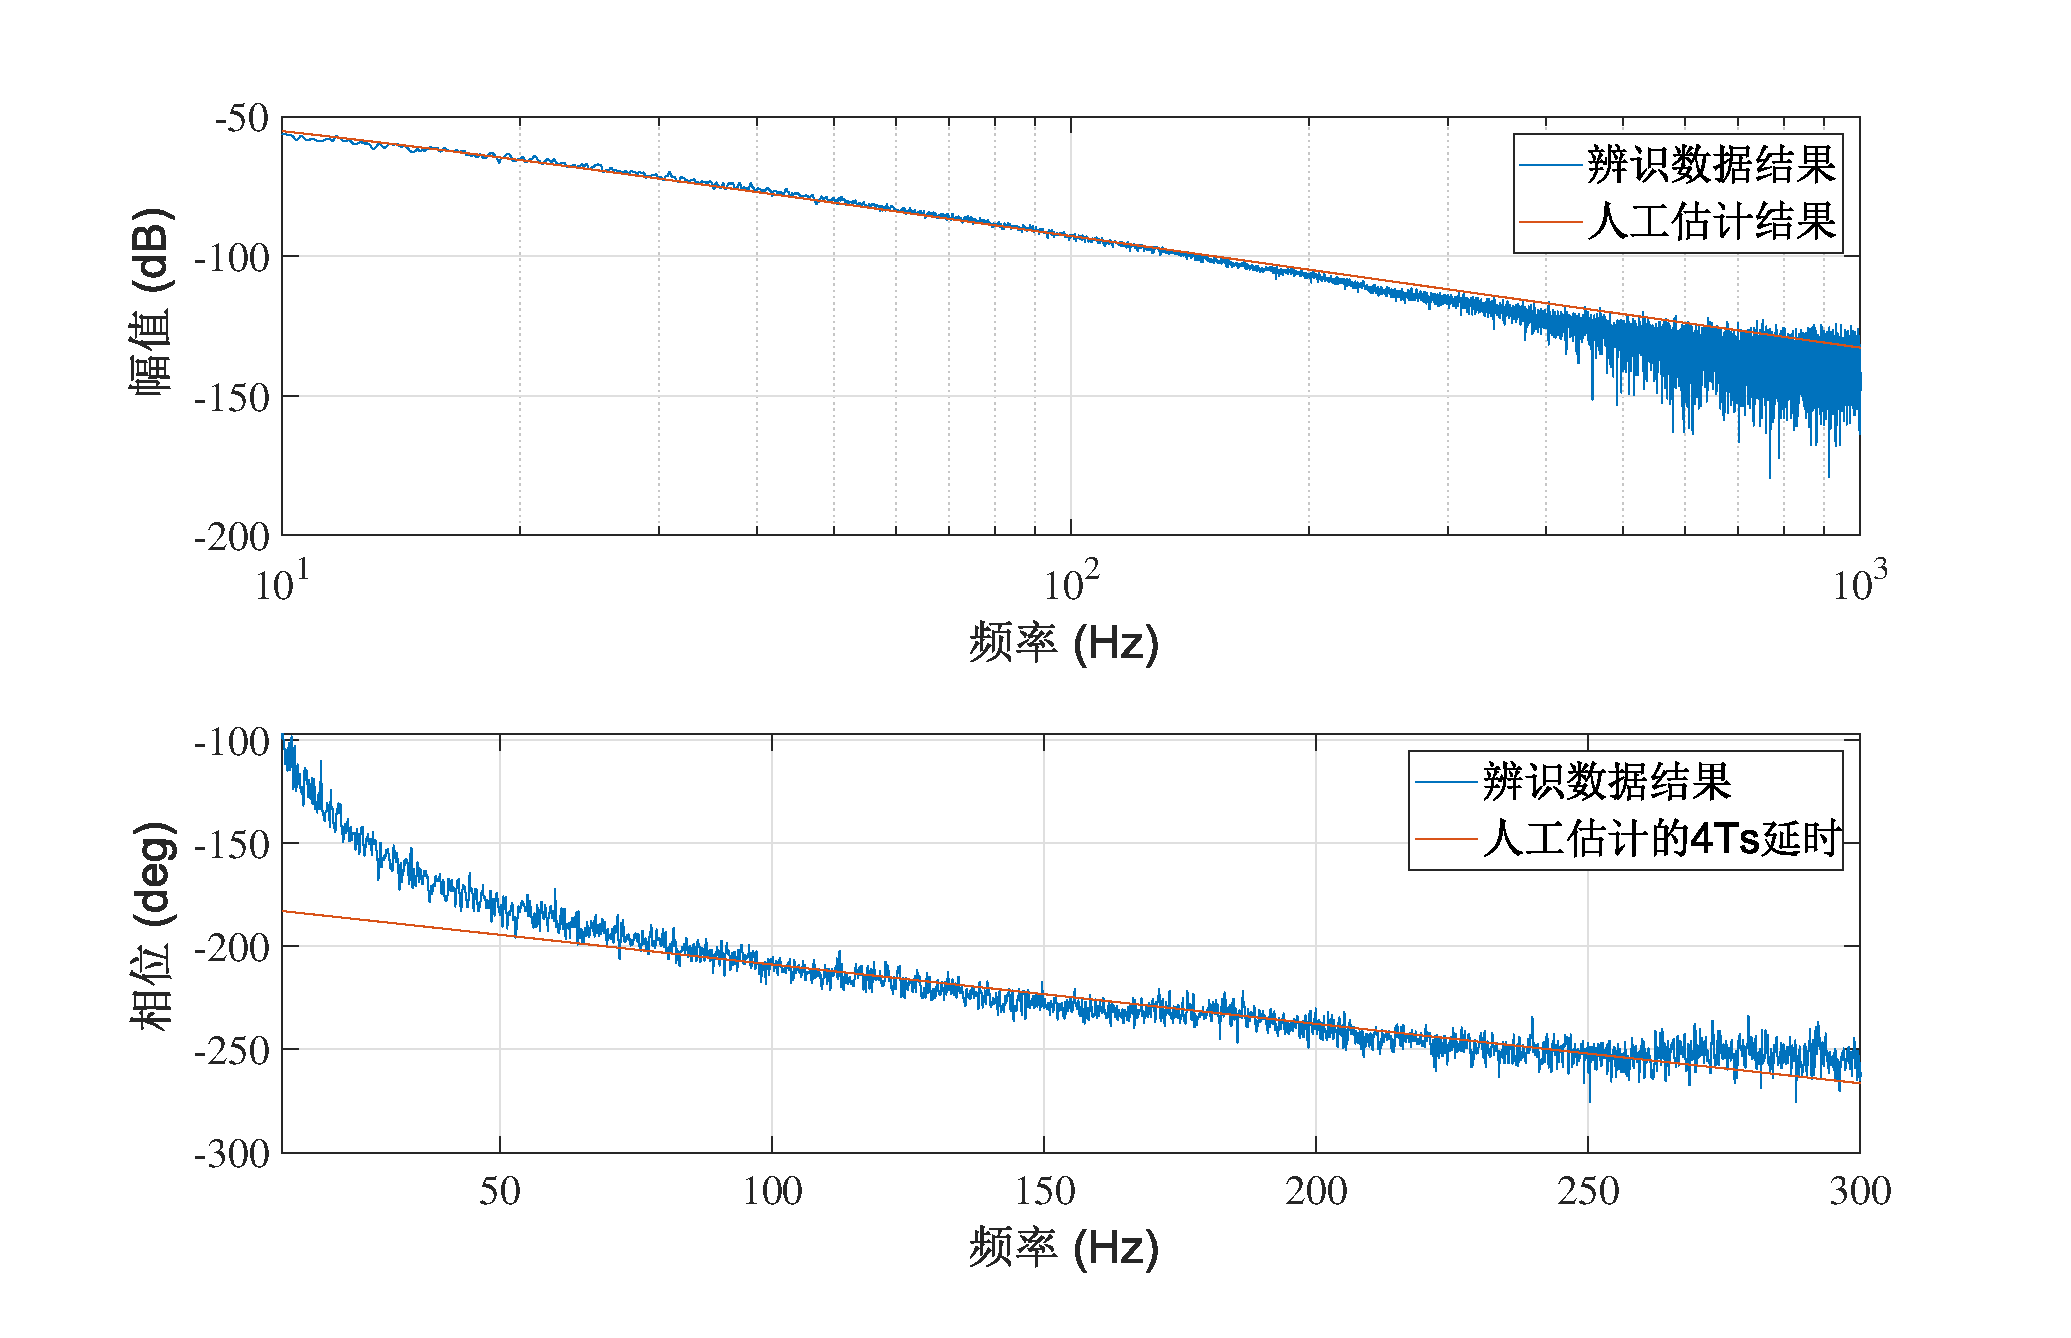
\includegraphics[width=12cm]{figures/辨识结果}
	\caption{辨识结果.}
	\label{辨识结果}
\end{figure}
图中,蓝色的线为实际辨识的数据,红色的线为辨识估计的数据。这里估计所采用的数学模型为最基础的二阶模型,如式(\ref{辨识公式})所示:
\begin{equation}
\label{辨识公式}
G(s)=\frac{1}{M_es^2+D_es}e^{-st_d}
\end{equation}
式中,由于辨识实际系统模型如图\ref{电机系统模型}所示,包含了驱动器部分,因此,辨识所得参数结果如下:

$M_e$为系统等效质量,这里为$\text{0.12$\,$Vs$^{2}$/m}$;

$D_e$为系统等效粘滞摩擦系数,这里为$\text{2.0$\,$Vs/m}$;

$t_d$为系统延时,这里为$\text{4$\,T_s$}$,即$\text{0.0008$\,$s}$。

从辨识结果来看,在300\,Hz以内,幅频曲线拟合的都比较好,超过300\,Hz,由于高频的未建模动态等因素,导致无法很好地拟合数据结果。相频曲线,从式(\ref{辨识公式})可知,估计采用的模型在$\text{s}$域内有两个极点,一个为0,另一个为$D_e/M_e$,即相位从-90°开始,在$\left|D_e/M_e\right|$\,Hz处下降90°,之后以斜率为$t_d$的直线变化,相对来说在300\,Hz以内,相频曲线较为理想。虽然高频无法很好地进行辨识,但辨识结果已经足以满足对于本文所涉及方法的要求,因为本文讨论的基于神经网络的一些方法对于模型的要求并不高,另外的一些补偿方法,也都会将模型的变化当做扰动的一种形式进行补偿。

此外,本文还对精密直线运动实验平台进行了定位力最大空间周期(即定位力的基频所对应的空间周期)的辨识,通过低速匀速运行,采集控制信号与位移信号,可以得到如图\ref{空间周期辨识}所示的结果,从图中很容易发现所标注的数据包含着定位力最大空间周期$\tau_{rip}=2\tau/3\,\text{mm}$的信息,其中$\tau$为实验平台PMLSM的极距($\tau=20\,\text{mm}$)。所标注出来的包含着几个非常常见的定位力的倍频所对应的空间周期,分别为$2\tau/3,\tau/3,\tau/4,\tau/6,2\tau/9$。
\begin{figure}[H]
	\centering
	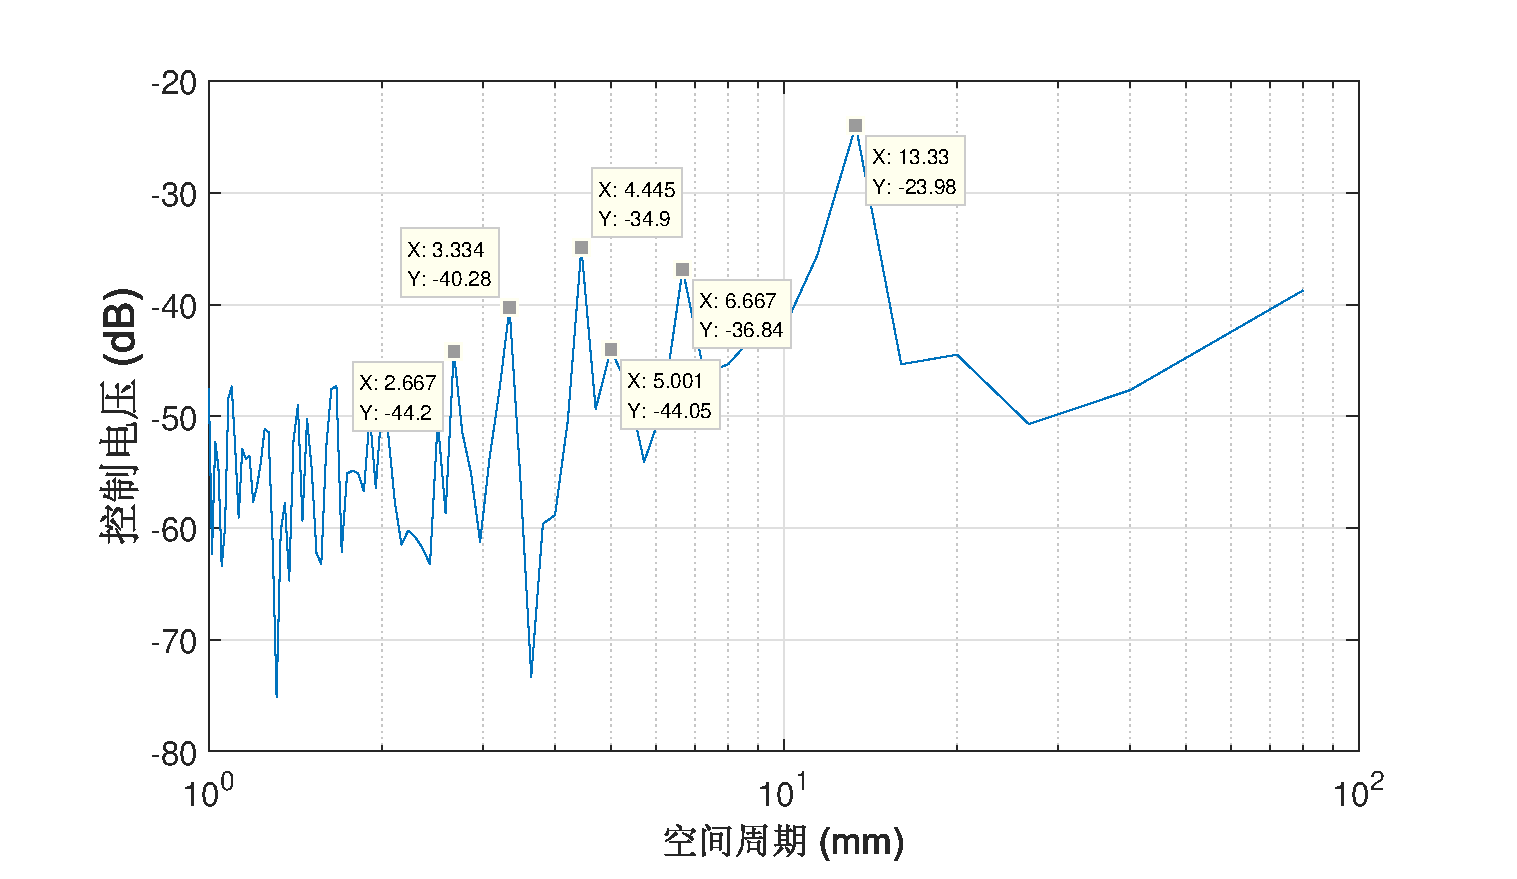
\includegraphics[width=12cm]{figures/空间周期辨识}
	\caption{定位力空间周期辨识.}
	\label{空间周期辨识}
\end{figure}
\section{本章小结}
本章首先介绍了精密直线运动平台系统工作原理,详细推导了PMLSMs的矢量变换控制原理。然后对精密直线运动平台动力学模型进行了详细介绍并提出了改进的扰动模型,其中,将系统扰动以集总扰动的形式进行了建模,为了方便后文控制方法的提出,进一步根据PMLSMs系统的特性,将集总扰动分为了时变的和时不变的两部分。此外,详细介绍了基于频率响应函数的系统辨识方法,详细介绍了离线开环辨识、闭环辨识和半闭环辨识三种辨识控制架构,并基于离线半闭环辨识控制架构对实验对象进行了辨识,得到了系统等效质量为$\text{0.12$\,$Vs$^{2}$/m}$,系统等效粘滞摩擦系数
为$\text{2.0\,Vs/m}$,系统延时为$\text{0.8$\,$ms}$,还对系统定位力的周期特性进行了辨识,得到其最大空间周期约为$13.33\,\text{mm}$,还可以发现,定位力的周期特性中,包含了2倍频、4倍频和6倍频的位置依赖扰动。这里系统模型特性为后续控制方法的研究提供了很好的基础。

%   \chapter{基于递推最小二乘的积分滑模控制方法研究}
\section{引言}
从第二章分析中可以知道,精密直线运动平台本质上也是一种非线性系统,尤其是其摩擦力、定位力、模型参数摄动、纹波扰动以及外部不确定扰动等均呈现出一定的非线性特性,因此,采用非线性的反馈控制器提高精密直线运动平台系统的整体控制性能显得很有必要,尤其是在超精密运动控制领域,抑制上述扰动带来的影响是提高运动控制性能的关键环节。近年来,滑模控制由于其控制律中含有具有开关特性的鲁棒项(符号函数及其变种),在处理PMLSMs诸多扰动因素时表现出优势\cite{wang2015modified,slotine1983tracking,burton1986continuous,tseng2010chattering,zhang2013design,lee2017adaptive}。但是,符号函数在原点附近的不连续会造成抖振,甚至可能造成系统不稳定或激发更多的不期望的模态,严重影响精密直线运动平台系统位置跟踪精度\cite{tseng2010chattering}。另一方面,由于缺乏对系统扰动的精确建模,传统的滑模控制方法在高速、高精度运动控制系统中不能完全满足要求,往往需要与额外的扰动补偿方法相结合。在精密直线运动平台控制系统中,前馈控制常常与反馈控制相结合,前者主要用来提高系统跟踪精度和补偿系统扰动,后者常用来维持系统稳定并一定程度上抑制系统的扰动,提高系统稳态精度。对于精密运动控制领域经常采用的三阶轨迹来说,前馈控制器主要在加减速段发挥作用,而反馈控制器主要在匀速段发挥作用。经典的前馈控制方法主要是基于系统的逆模型,但是往往需要提前辨识系统的模型,而且对模型辨识的精度要求极高,对于复杂的系统往往很难做到精确辨识,因此自适应的逆模型前馈控制显得很有必要。

本章首先介绍了滑模控制和递推最小二乘(Recursive Least Square, RLS)算法的基本原理,然后用积分滑模控制(Integral Sliding Mode Control, ISMC)作为反馈部分,用RLS实现逆模型的自适应前馈控制。为了能够补偿定位力带来的扰动,进一步对基于RLS的自适应逆模型前馈方法进行了改进,提出了一种基于改进型RLS的积分滑模控制方法,该方法将定位力的主要频率部分引入到RLS的回归向量中,从而进一步提高系统位置跟踪精度。
\section{滑模控制基本原理}
考虑单输入动态系统\cite{slotine2006应用非线性控制}
\begin{equation}
\label{4单输入动态系统}
x^{(n)}=f(\textbf{\textit{x}})+b(\textbf{\textit{x}})u
\end{equation}
式中,标量$x$是控制系统输出(如精密直线运动平台的位置),标量$u$是控制信号输入(比如电机的出力),向量$\textbf{\textit{x}}=[x,\dot{x},\dots,x^{n-1}]^T$为状态向量。$f(\textbf{\textit{x}})$通常表示一个非线性函数,用来表示系统的扰动,虽然不能精确知道,但一般都认为它的上界是$\textbf{\textit{x}}$的连续函数。$b(\textbf{\textit{x}})$也认为不能精确已知,但是其不确定性也认为是有界的,比如PMLSMs模型参数摄动等。

为了使有限控制$u$实现较为理想的跟踪任务,系统的期望状态的初始值$\textbf{\textit{x}}_d(0)$必须满足
\begin{equation}
\label{初态}
\textbf{\textit{x}}_d(0)=\textbf{\textit{x}}(0)
\end{equation}
即当$t=0$时控制系统输出与目标轨迹一致,这一条件在实际精密运动控制中基本都会满足,因为系统的位置和速度不会突变。

记跟踪误差为$e=x_d-x$,则跟踪误差向量为 $\textbf{\textit{e}}=\textbf{\textit{x}}_d-\textbf{\textit{x}}=[e \quad\dot {e} \quad\cdots \quad e^{n-1}]^T$。用标量方程$s(\textbf{\textit{e}};t)=0$定义n维状态空间中的滑模曲面$S(t)$
\begin{equation}
\label{滑模面0}
s(\textbf{\textit{e}},t)=\left(\frac{\text{d}}{\text{dt}}+\lambda\right)^{n-1}\textbf{\textit{e}}
\end{equation}
式中,$\lambda$为一正常数。$n$表示系统的阶数,比如机械系统,大部分会是二阶系统,即$n=2$,此时
\begin{equation}
\label{滑模面1}
s=\lambda e+\dot{e}
\end{equation}
即$s$仅是状态轨迹,即系统跟踪位置误差和速度误差的线性加权;$\lambda$为一正常数。


给定初始状态(\ref{初态}),跟踪问题$\textbf{\textit{x}}\equiv\textbf{\textit{x}}_d$则等价于当$t$\textgreater$0$时,通过一定的控制手段使系统状态轨迹能够始终停留在曲面$S(t)$上。实际上$s\equiv0$本质上为一种线性微分方程的表示,假定系统状态轨迹的初态满足式(\ref{初态}),则其唯一解为$\tilde{\textbf{\textit{x}}}\equiv0$。因此,通过一定的控制方式实现跟踪$n$维向量$\textbf{\textit{x}}_d$的问题可巧妙地转化为如何使标量$s$恒为零的问题。

更进一步,通过选择式(\ref{4单输入动态系统})中的控制信号$u$,使得状态轨线在曲面$S(t)$之外满足下式
\begin{equation}
\label{收敛条件}
\frac{1}{2}\frac{\text{d}}{\text{dt}}s^2\leq-\eta\left|s\right|
\end{equation}
从而保证$s$恒为零的问题简化为一阶问题,其中$\eta$为一正常数。如图\ref*{滑动条件}所示,系统状态轨线只要能够满足式(\ref{收敛条件}),系统状态轨线就会不断趋向于曲线$S(t)$,曲面$S(t)$就可以认为是一个不变集。系统状态轨线沿曲面$S(t)$运动的状态我们称为滑动模态。
%满足式(\ref{收敛条件})的曲面$S(t)$称为滑动曲面,当系统状态轨迹进入滑动曲面后,我们可以说系统进入了滑动模态,或滑动模。
\begin{figure}[H]
	\centering
	\includegraphics[width=10cm]{figures/滑动条件.pdf}
	\caption{滑动条件}
	\label{滑动条件}
\end{figure}
\begin{comment}
实际上,即使式(\ref*{初态})不满足,即初始时刻,系统输出与系统目标轨迹不一致,也就是说,系统不满足零状态,系统轨线仍然能够在小于$s(t=0)/\eta$的有限时间内到达曲面$S(t)$。总的来说,这种通过设计滑模面$S(t)$,并合理设计控制律$u$以使系统状态轨迹收敛到滑模面上的方法,成为滑模控制,是一种有效的容易实现的鲁棒控制方法。
\end{comment}
\section{递推最小二乘原理}
在介绍递推最小二乘原理之前,有必要先介绍最小二乘法。最小二乘法主要解决的问题是,对于像式(\ref{最小二乘})一样的表示,
\begin{equation}
\label{最小二乘}
y=\left[\begin{matrix}
x_{1} & \cdots & x_{n}
\end{matrix}\right]\left[\begin{matrix}
\theta_{1} \\
\vdots \\
\theta_{n}
\end{matrix}\right]
\end{equation}
其中$x$和$y$为一系列观测得到的数据,通过观测得到的$x$和$y$,求解其对应的估计参数$\symbf{\Theta}$的过程。可以用矩阵表示如下
\begin{equation}
\left[\begin{matrix}
y_{1} \\
\vdots \\
y_{k}
\end{matrix}\right]=\left[\begin{matrix}
\symbf{\phi}_{1}^{T} \\
\vdots \\
\symbf{\phi}_{k}^{T}
\end{matrix}\right] \symbf{\Theta}
\end{equation}
式中,
$k$表示观测到的数据个数;
$\symbf{\phi}_{i}^{T}=\left[\begin{matrix}x_{1}^{i} & \cdots & x_{n}^{i}\end{matrix}\right] \in \mathbb{R}^{1 \times n}$,表示第$i$组观测数据的输入量;

$y_i$表示第$i$组观测数据的输出量;

$\symbf{\Theta}=\left[\begin{matrix}\theta_{1} \\ \vdots \\ \theta_{n}\end{matrix}\right] \in \mathbb{R}^{n \times 1}$,为待估计参数。

记$\symbf{\Phi}_{k}=\left[\begin{matrix}\symbf{\phi}_{1}^{T} \\ \vdots \\ \symbf{\phi}_{k}^{T}\end{matrix}\right] \in \mathbb{R}^{k \times n}, \symbf{Y}_{k}=\left[\begin{matrix}y_{1} \\ \vdots \\ y_{k}\end{matrix}\right] \in \mathbb{R}^{k \times 1}$,则有
\begin{equation}
\label{3.8}
\symbf{\Phi}_{k}^{T}\left(\symbf{Y}_{k}-\symbf{\Phi}_{k} \hat{\symbf{\Theta}}_{k}\right)=0
\end{equation}
则通过方程(\ref{3.8}),即可求得最小二乘参数$\symbf{\Theta}_k$的估计,
\begin{equation}
\label{3.9}
\hat{\symbf{\Theta}}_{k}=\left(\symbf{\Phi}_{k}^{T} \symbf{\Phi}_{k}\right)^{-1} \symbf{\Phi}_{k}^{T} \symbf{Y}_{k}
\end{equation}
通过上述过程,可以发现,如果我们能够得到$x$和$y$的观测值,我们可以通过最小二乘方法求出$y$和$x$之间的函数关系。但是最小二乘法要求计算之前就能够得到所有的观测值,也就是说所有的数据都要提前准备好,这要求较大的存储空间,也影响计算速度,不利于实时在线的计算和补偿。因此,递推最小二乘应运而生。

递推最小二乘原理的根本目的是希望能够得到一种估计值的递推形式,比如$\hat{\symbf{\Theta}}_k=\hat{\symbf{\Theta}}_{k-1}+\Delta\hat{\symbf{\Theta}}_k$。下面是详细的推导过程:

最小二乘法的一般解如式(\ref{3.9})所示,这里分别表示$\symbf{\Phi}_{k}^{T} \symbf{\Phi}_{k}$和$\symbf{\Phi}_{k}^{T} \symbf{Y}_{k}$,令$\symbf{P}_{k}^{-1}=\symbf{\Phi}_{k}^{T} \symbf{\Phi}_{k}$,则有
\begin{equation}
\label{公式1}
\begin{aligned}
\symbf{\Phi}_{k}^{T} \symbf{\Phi}_{k}&=\left[\begin{matrix}
\symbf{\phi}_{1} & \cdots & \symbf{\phi}_{k}
\end{matrix}\right]\left[\begin{matrix}
\symbf{\phi}_{1}^{T} \\
\vdots \\
\symbf{\phi}_{k}^{T}
\end{matrix}\right]\\
&=\sum_{i=1}^{k} \symbf{\phi}_{i} \symbf{\phi}_{i}^{T}\\
&=\sum_{i=1}^{k-1} \symbf{\phi}_{i} \symbf{\phi}_{i}^{T}+\symbf{\phi}_{k} \symbf{\phi}_{k}^{T}\\
&=\symbf{P}_{k-1}^{-1}+\symbf{\phi}_{k} \symbf{\phi}_{k}^{T}
\end{aligned}
\end{equation}
同时,
\begin{equation}
\label{公式2}
\begin{aligned}
\symbf{\Phi}_{k}^{T} \symbf{Y}_{k}&=\left[\begin{matrix}
\symbf{\phi}_{1} & \cdots & \symbf{\phi}_{k}
\end{matrix}\right]\left[\begin{matrix}
y_{1} \\
\vdots \\
y_{k}
\end{matrix}\right]\\
&=\sum_{i=1}^{k} \symbf{\phi}_{i} y_{i}\\
&=\sum_{i=1}^{k-1} \symbf{\phi}_{i} y_{i}+\symbf{\phi}_{k} y_{k}\\
&=\symbf{\Phi}_{k-1}^{T} \symbf{Y}_{k-1}+\symbf{\phi}_{k} y_{k}
\end{aligned}
\end{equation}

此外,根据最小二乘法的一般解可以得到
\begin{equation}
\label{公式3}
\begin{matrix}
\hat{\symbf{\Theta}}_{k-1}=\left(\symbf{\Phi}_{k-1}^{T} \symbf{\Phi}_{k-1}\right)^{-1} \symbf{\Phi}_{k-1}^{T} \symbf{Y}_{k-1} \\
\Rightarrow \hat{\symbf{\Theta}}_{k-1}=\symbf{P}_{k-1} \symbf{\Phi}_{k-1}^{T} \symbf{Y}_{k-1} \\
\Rightarrow \symbf{P}_{k-1}^{-1} \hat{\symbf{\Theta}}_{k-1}=\symbf{\Phi}_{k-1}^{T} \symbf{Y}_{k-1}
\end{matrix}
\end{equation}

结合公式(\ref{公式1})$\sim$公式(\ref{公式3}),再次回顾最小二乘法的一般解,可以得出下面的推导
\begin{equation}
\begin{aligned}
\hat{\symbf{\Theta}}_{k}&=\left(\symbf{\Phi}_{k}^{T} \symbf{\Phi}_{k}\right)^{-1} \symbf{\Phi}_{k}^{T} \symbf{Y}_{k}\\
%&=\symbf{P}_{K} \symbf{\Phi}_{k}^{T} \symbf{Y}_{k}\\
&=\symbf{P}_{k}\left(\symbf{\Phi}_{k-1}^{T} \symbf{Y}_{k-1}+\symbf{\phi}_{k} \symbf{y}_{k}\right) \\
&=\symbf{P}_{k}\left(\symbf{P}_{k-1}^{-1} \hat{\symbf{\Theta}}_{k-1}+\symbf{\phi}_{k} \symbf{y}_{k}\right) \\
&=\symbf{P}_{k}\left[\left(\symbf{P}_{k}^{-1}-\symbf{\phi}_{k} \symbf{\phi}_{k}^{T}\right) \hat{\symbf{\Theta}}_{k-1}+\symbf{\phi}_{k} \symbf{y}_{k}\right] \\
%&=\hat{\symbf{\Theta}}_{k-1}-\symbf{P}_{k} \symbf{\phi}_{k} \symbf{\phi}_{k}^{T} \hat{\symbf{\Theta}}_{k-1}+\symbf{P}_{k} \symbf{\phi}_{k} \symbf{y}_{k}\\
&=\hat{\symbf{\Theta}}_{k-1}+\symbf{P}_{k} \symbf{\phi}_{k}\left(y_{k}-\symbf{\phi}_{k}^{T}\hat{\symbf{\Theta}}_{k-1}\right)\\
&=\hat{\symbf{\Theta}}_{k-1}+\symbf{K}_{k} \varepsilon_{k}\\
\end{aligned}
\end{equation}
至此,估计参数写成了$\hat{\symbf{\Theta}}_{k}=\hat{\symbf{\Theta}}_{k-1}+\Delta\symbf{\Theta}$的形式,其中$\Delta\symbf{\Theta}=\symbf{K}_k\varepsilon_{k}$。

综合上述的推导过程,这里可以进一步地给出递推最小二乘法的原理公式:
\begin{equation}
\label{RLS}
\left\{
\begin{aligned}
\hat{\symbf{\Theta}}_{k}&=\hat{\symbf{\Theta}}_{k-1}+\symbf{K}_{k} \varepsilon_{k}\\
\symbf{K}_{k}&=\symbf{P}_{k} \symbf{\phi}_{k}\\
\varepsilon_{k}&={y_{k}}-{\symbf{\phi}_{k}^{T} \hat{\symbf{\Theta}}_{k-1}}\\
\symbf{P}_{k}&=\left(\symbf{P}_{k-1}^{-1}+\symbf{\phi}_{k} \symbf{\phi}_{k}^{T}\right)^{-1}
\end{aligned}
\right.
\end{equation}
这里需要说明的是,$y_k$为标量、$\symbf{\phi}_{k}^{T}$、$\symbf{\Theta}_k$、$\symbf{\Theta}_{k-1}$都为向量。值得注意的是,公式(\ref{RLS})还无法通过编程实现递推最小二乘算法进行参数$\symbf{\Theta}$的估计。还要对其中的$\symbf{P}_k$进行进一步地求解。这里首先给出一个矩阵引逆定理(证明略):
假设矩阵$\symbf{A}\in \mathbb{C}^{N\times N}$,$\symbf{C}\in\mathbb{C}^{N\times N}$,均为非奇异矩阵,矩阵$\symbf{B}\in\mathbb{C}^{N\times M}$,$\symbf{D}\in\mathbb{C}^{M\times N}$,则矩阵$\symbf{A}+\symbf{BCD}$具有逆矩阵:
\begin{equation}
\label{引逆定理}
[\symbf{A}+\symbf{B C D}]^{-1}=\symbf{A}^{-1}-\symbf{A}^{-1} \symbf{B}\left[\symbf{C}^{-1}+\symbf{D} \symbf{A}^{-1} \symbf{B}\right]^{-1} \symbf{D} \symbf{A}^{-1}
\end{equation}
根据矩阵引逆定理(\ref{引逆定理}),
设 $\symbf{A}=\symbf{P}_{K-1}^{-1}, \symbf{B}=\symbf{\phi}_{k}, \symbf{C}=1, \symbf{D}=\symbf{\phi}_{k}^{T}$
则有
\begin{equation}
\label{逆}
\begin{aligned}
\symbf{P}_{k}&=\left(\symbf{P}_{k-1}^{-1}+\symbf{\phi}_{k} \symbf{\phi}_{k}^{T}\right)^{-1}\\
&=[\symbf{A}+\symbf{B C D}]^{-1}\\
&=\symbf{A}^{-1}-\symbf{A}^{-1} \symbf{B}\left[\symbf{C}^{-1}+\symbf{D} \symbf{A}^{-1} \symbf{B}\right]^{-1} \symbf{D} \symbf{A}^{-1}\\
&=\symbf{P}_{k-1}-\symbf{P}_{k-1} \symbf{\phi}_{k}\left[1+\symbf{\phi}_{k}^{T} \symbf{P}_{k-1} \symbf{\phi}_{k}\right]^{-1} \symbf{\phi}_{k}^{T} \symbf{P}_{k-1}\\
&=\symbf{P}_{k-1}-\frac{\symbf{P}_{k-1} \symbf{\phi}_{k} \symbf{\phi}_{k}^{T} \symbf{P}_{k-1}}{1+\symbf{\phi}_{k}^{T} \symbf{P}_{k-1} \symbf{\phi}_{k}}
\end{aligned}
\end{equation}

将式(\ref{逆})带入式(\ref{RLS}),可以得到最终的递推最小二乘算法:
\begin{equation}
\label{RLS1}
\left\{
\begin{aligned}
\hat{\symbf{\Theta}}_{k}&=\hat{\symbf{\Theta}}_{k-1}+\symbf{K}_{k} \varepsilon_{k}\\
\symbf{K}_{k}&=\symbf{P}_{k} \symbf{\phi}_{k}\\
\varepsilon_{k}&={y_{k}}-{\symbf{\phi}_{k}^{T}\hat{\symbf{\Theta}}_{k-1}}\\
\symbf{P}_{k}&=\symbf{P}_{k-1}-\frac{\symbf{P}_{k-1} \symbf{\phi}_{k} \symbf{\phi}_{k}^{T} \symbf{P}_{k-1}}{1+\symbf{\phi}_{k}^{T} \symbf{P}_{k-1} \symbf{\phi}_{k}}
\end{aligned}
\right.
\end{equation}
其中,

$y_k$为输出观测值;

$\symbf{\phi}_k$为输入观测向量,也称回归向量;

$\hat{\symbf{\Theta}}_{k}$为待估计参数向量;

$\symbf{P}_k$为更新律。
至此,所得到的递推最小二乘算法可以直接通过编程实现。


\section{基于传统递推最小二乘的前馈控制器设计}
在光刻机工件台与掩模台运动控制系统中,由于高分辨率和高产率的需求,常常希望精密直线运动平台加速段的精度更高、整定时间更短,这时,往往只靠反馈控制器不能很好地实现这一目的,因此,将前馈补偿与反馈控制相结合成为了一种较为流行的控制架构。经典的前馈补偿方式为系统逆模型前馈,通过事先辨识好系统的模型参数,然后通过逆模型前馈的方式计算得到需要的力。但是这种方式,需要对模型参数事先进行辨识,而且要求的辨识精度较高,往往需要付出额外的人力物力成本。一种较好的策略是通过在线自适应的方式调整系统的逆模型前馈参数\cite{butler2012adaptive},这样对于提前辨识的参数精度要求不高,只需要一个粗略的初始值即可实现逆模型自适应前馈控制,本节重点研究基于递推最小二乘方法进行逆模型自适应前馈的策略,并将之与积分滑模控制相结合,实现精密直线运动平台的高性能控制。

传统递推最小二乘积分滑模系统控制框图如图\ref{传统RLS}所示,主要包含自适应逆模型前馈与积分滑模反馈两部分,下面具体介绍基于传统递推最小二乘的前馈控制器的设计。
% TODO: \usepackage{graphicx} required
\\
\begin{figure}[H]
	\centering
	\includegraphics[width=12cm]{figures/RLSISMC2.pdf}
	\caption{传统递推最小二乘的积分滑模控制系统框图}
	\label{传统RLS}
\end{figure}

%\subsection{基于传统递推最小二乘的前馈控制器设计}

以经典的集中质量模型$1/(M_es^2+D_es+K_e)$为例,逆模型前馈控制信号可以表示为
\begin{equation}
\label{传统逆模型前馈}
u_{ff}=(M_es^2+D_es+K_e)p_d
\end{equation}
式中,$p_d$为系统位置参考轨迹。$M_e$、$D_e$和$K_e$为系统逆模型待确定的参数,$s$为拉普拉斯算子,表示微分。

如果将逆模型待确定的参数表示为向量的形式$\symbf{\Theta}=[M_e\,\, D_e\,\, K_e]^{T}$,则根据式(\ref{RLS1}),$\symbf{\Theta}$可以被估计为
\begin{equation}
\label{3.20}
\hat{\symbf{\Theta}}_{k}=\hat{\symbf{\Theta}}_{k-1}+\symbf{P}_{k} \symbf{\phi}_{k}\varepsilon_{k}
\end{equation}
式中,

$\hat{\symbf{\Theta}}_{k}$表示待确定参数向量的估计值;

$\symbf{P}_k$为自适应更新律,为一矩阵,可以表示为$\symbf{P}_{k}=\symbf{P}_{k-1}-\frac{\symbf{P}_{k-1} \symbf{\phi}_{k} \symbf{\phi}_{k}^{T} \symbf{P}_{k-1}}{1+\symbf{\phi}_{k}^{T} \symbf{P}_{k-1}\symbf{\phi}_{k}}$;

$\symbf{\phi}_{k}$为递推最小二乘的回归向量,即基向量,可以表示为$\symbf{\phi}_{k}=\left[\frac{d^{2} p_d}{d t^{2}} \,\,\frac{d p_d}{d t} \,\,p_d \right]^{T}$,这里指系统的三阶参考轨迹;

$\varepsilon_{k}$表示估计误差。

一旦$\symbf{\Theta}_k$的估计值$\hat{\symbf{\Theta}_k}$得到,就可以通过计算得出前馈控制器的估计输出指令
\begin{equation}
\label{3.21}
\hat{u_{ff}}=\hat{\symbf{\Theta}_k}^{T}\symbf{\phi}_{k}
\end{equation}
理想前馈控制器输出指令与估计得到的输出指令之间的差值可以表示为
\begin{equation}
\label{3.22}
\varepsilon_{k}^{'}=u_{ff}-\hat{u_{ff}}=\left[\symbf{\Theta}_k-\hat{\symbf{\Theta}_k}\right]^{T}\symbf{\phi}_{k}
\end{equation}
结合式(\ref{3.20})和式(\ref{3.22})以及文献\cite{landau1980extension}中定理2.1所表示的系统,$\varepsilon_{k}^{'}$又可假设为
\begin{equation}
\label{3.23}
\varepsilon_{k}^{'}=u_{ff}-\hat{u_{ff}}=Q\left[\Theta_k-\hat{\Theta_{k}}\right]^{T}\phi_{k}
\end{equation}
式中,$Q$为一离散的有理分式,根据波波夫超稳定性理论\cite{landau1980extension},如果$Q^{'}=Q-\frac{\lambda}{2}\,(0<\lambda<1)$严格正定,那么不管参数向量的估计初值$\hat{\symbf{\Theta}_0}$和自适应更新律初值$\symbf{P}_0$为何值,都有$\varepsilon_{k}^{'}$有界且
\begin{equation}
\label{3.24}
\lim _{k \rightarrow \infty} \varepsilon_{k}^{'}=0
\end{equation}

根据式(\ref{3.22})和式(\ref{3.23}),不难发现,在这里离散的有理传递函数$Q=1$,而且$Q^{'}=Q-\frac{\lambda}{2}>\frac{1}{2}$严格正定,因此,基于式(\ref{3.25})的递推最小二乘估计算法能够保证估计参数的收敛性。从图\ref{RLSISMC}
中可以看到,自适应前馈部分并未包含在系统的反馈回路中,因此,只要能够保证自身参数的收敛性,基于递推最小二乘估计的自适应前馈部分并不影响整个系统的闭环稳定性,闭环稳定性完全由积分滑模控制部分决定。
\begin{comment}
\subsection{基于积分滑模的反馈控制器设计}

精密直线运动平台的系统模型如式(\ref{2.14})所示,
$$
\begin{aligned}
\ddot{p}&=({{A}_{n}}+\Delta A)u_{fb}+L \\
&={A}_{n}u_{fb}+H  
\end{aligned}
$$
这里假设总扰动$H$有界,即$H\le\mu$,$\mu$为一正常数。$u_{fb}$表示反馈控制指令。

定义系统位置跟踪误差为
\begin{equation}
\label{3.25}
e=p_d-p
\end{equation}
可以得到误差对时间的导数为
\begin{equation}
\label{3.26}
\dot{e}=\dot{p_d}-\dot{p}
\end{equation}
滑模控制部分的设计主要包括两部分:滑模面的设计和控制律的设计。
这里设计滑模面为含积分项的滑模面
\begin{equation}
\label{3.27}
s=\lambda e+\beta\int_{}^{}e\text{d}t+\dot{e}
\end{equation}
式中,$\lambda$和$\beta$均为正常数。

根据式(\ref{3.26})和(\ref{3.27}),可以得出滑模面对时间的一阶导数为
\begin{equation}
\label{3.28}
\begin{aligned}
\dot{s}&=\lambda \dot{e}+\beta e+\ddot{e} \\ 
&=\lambda\dot{e}+\beta e+{{{\ddot{p}}}_{d}}-\ddot{p} \\ 
&=\lambda \dot{e}+\beta e+{{{\ddot{p}}}_{d}}-{{A}_{n}}u_{fb}-H  
\end{aligned}
\end{equation}
这里考虑到系统状态轨线的初始状态可能与目标轨迹的初始状态不一致,即系统可能不是零状态,因此需要一定的到达阶段才能保证系统状态轨线收敛到滑模面,为了方便,选定到达阶段的趋近律为等速趋近律
\begin{equation}
\label{3.29}
\dot{s}=-\eta\text{sgn}(s)
\end{equation}
式中,

$\text{sgn}(\cdot)$为符号函数;

$\eta$为正常数,满足$\eta\ge\mu$,主要决定到达阶段的趋近速率以及滑模控制的鲁棒性。

另一方面,设计滑模控制律为
\begin{equation}
\label{3.30}
u_{fb}=\frac{1}{A_n}\left(\lambda \dot{e}+\beta e+\ddot{p_d}+\eta\text{sgn}(s)\right)
\end{equation}
将式(\ref{3.30})代入式(\ref{3.28}),可得
\begin{equation}
\label{3.31}
\dot{s}=-\eta \text{sgn}(s)-H
\end{equation}

如前面提到的,基于递推最小二乘的积分滑模控制系统的闭环稳定性取决于积分滑模控制部分,这里为了证明其稳定性,根据Lyapunov稳定性理论,选择Lyapunov函数
\begin{equation}
\label{3.32}
V=\frac{1}{2}s^2
\end{equation}
两边对时间求导,即可得
\begin{equation}
\label{3.33}
\dot{V}=s\dot{s}
\end{equation}
将式(3.31)代入(3.33)中可以得到
\begin{equation}
\label{3.34}
\begin{aligned}
\dot{V}&=-\eta s\text{sgn}(s)-sH\\
&=-\eta\left|s\right|-sH\\
&\leq-\eta\left|s\right|+\mu\left|s\right|\\
&\leq-(\eta-\mu)\left|s\right|\\
&\leq 0
\end{aligned}
\end{equation}
取$\dot{V}\equiv0$,则$s\equiv0$,由LaSalle不变集定理可知,当$t\to\infty,s\to0$。至此,积分滑模反馈控制部分的渐近稳定性得以证明,反馈控制部分也设计完毕。
\end{comment}

\section{基于改进型递推最小二乘的积分滑模控制器设计}
\begin{comment}
在精密直线运动平台中,采用传统的基于递推最小二乘的积分滑模控制方法能够提高系统的位置跟踪精度,尤其是基于递推最小二乘的自适应逆模型前馈,能够有效地提高加速段的跟踪精度,同时减小系统从加速段进入匀速段的整定时间。但是正如第二章讨论的一样,由于精密直线运动平台本身的诸多非线性因素的影响,要进一步地提高系统的位置跟踪精度和扰动抑制能力,仅依赖逆模型前馈的积分滑模控制还有改进的空间。
\end{comment}




本节重点针对精密直线运动平台的定位力带来的扰动,在自适应前馈阶段引入了定位力的最大空间周期对应的扰动,对原有递推最小二乘的回归向量进行了改进,改进后的回归向量为$\symbf{\phi}_{k}^{'}=\left[\frac{d^{2} p}{d t^{2}} \,\,\frac{d p}{d t} \,\,p \,\,\text{sin}\left(2\pi p/\tau_m\right)\,\,\text{cos}\left(2\pi p/\tau_m\right)\right]^{T}$,其中,$\tau_m=2\tau/3=40/3\,\text{mm}$。改进之后的递推最小二乘可以分为两个部分:一是逆模型前馈部分,主要用来提高系统的瞬态响应速度;另一个是定位力补偿部分,用来补偿位置依赖的扰动对位置跟踪精度的影响。两部分都通过改进的递推最小二乘估计方法进行自适应调节,改进递推最小二乘积分滑模控制系统框图如图\ref{RLSISMC}所示。下面详细地介绍各部分的设计过程。
\begin{figure}[H]
	\centering
	\includegraphics[width=12cm]{figures/RLSISMC系统框图.pdf}
	\caption{改进递推最小二乘积分滑模控制系统框图}
	\label{RLSISMC}
\end{figure}

\subsection{基于改进型递推最小二乘的前馈控制器设计}
在工程实际中,还存在一种带遗忘因子的递推最小二乘算法\cite{butler2012adaptive}:
\begin{equation}
\label{RLS2}
\left\{
\begin{aligned}
\hat{\symbf{\Theta}}_{k}&=\hat{\symbf{\Theta}}_{k-1}+\symbf{K}_{k} \varepsilon_{k}\\
\symbf{K}_{k}&=\symbf{P}_{k} \symbf{\phi}_{k}\\
\varepsilon_{k}&={y_{k}}-{\symbf{\phi}_{k}^{T}\hat{\symbf{\Theta}}_{k-1}}\\
\symbf{P}_{k}&=\frac{1}{\zeta}\left(\symbf{P}_{k-1}-\frac{\symbf{P}_{k-1} \symbf{\phi}_{k} \symbf{\phi}_{k}^{T} \symbf{P}_{k-1}}{\zeta+\symbf{\phi}_{k}^{T} \symbf{P}_{k-1} \symbf{\phi}_{k}}\right)
\end{aligned}
\right.
\end{equation}
式中,$\zeta$为遗忘因子,$0<\zeta<1$,一般取0.98$\sim$0.999。本节改进型递推最小二乘的自适应更新律即采用式(\ref{RLS2})中的更新律。


因为改进后的回归向量为$\symbf{\phi}_{k}^{'}=\left[\frac{d^{2} p}{d t^{2}} \,\,\frac{d p}{d t} \,\,p \,\,\text{sin}\left(2\pi p/\tau_m\right)\,\,\text{cos}\left(2\pi p/\tau_m\right)\right]^{T}$,其中,$\tau_m=2\tau/3=40/3\,\text{mm}$。
这里将待确定的参数向量表示为$\symbf{\Theta}^{'}=[M_e\,\, D_e\,\, K_e\,\,a_1\,\,b_1]^{T}$,则根据式(\ref{RLS1}),$\Theta$可以被估计为
\begin{equation}
\label{3.25}
\hat{\symbf{\Theta}_{k}^{'}}=\hat{\symbf{\Theta}_{k-1}^{'}}+\symbf{P}_{k}^{'} \symbf{\phi}_{k}^{'}\varepsilon_{k}^{'}
\end{equation}
%式中,
%
%$\hat{\Theta_{k}^{'}}$表示待确定参数向量的估计值;
%
%$P_k^{'}$为自适应更新律,为一矩阵,可以表示为$P_{k}^{'}=P_{k-1}^{'}-\frac{P_{k-1}^{'} \phi_{k}^{'} {\phi_{k}^{'}}^{T} P_{k-1}^{'}}{1+{\phi_{k}^{'}}^{T} P_{k-1}^{'}\phi_{k}^{'}}$;
%
%$\phi_{k}^{'}$为改进后的回归向量;
%
%$\varepsilon_{k}^{'}$表示估计误差。

一旦$\Theta_k^{'}$的估计值$\hat{\Theta_k^{'}}$得到,就可以通过计算得出前馈控制器的估计输出指令
\begin{equation}
\label{3.26}
\hat{u_{ff}^{'}}=\hat{\symbf{\Theta}_k^{'}}^{T}\symbf{\phi}_{k}^{'}
\end{equation}


\subsection{基于积分滑模的反馈控制器设计}

精密直线运动平台的系统模型如式(\ref{2.14})所示,
$$
\begin{aligned}
\ddot{p}&=({{A}_{n}}+\Delta A)u_{fb}+L \\
&={A}_{n}u_{fb}+H  
\end{aligned}
$$
这里假设总扰动$H$有界,即$H\le\mu$,$\mu$为一正常数。$u_{fb}$表示反馈控制指令。

定义系统位置跟踪误差为
\begin{equation}
\label{3.27}
e=p_d-p
\end{equation}
可以得到误差对时间的导数为
\begin{equation}
\label{3.28}
\dot{e}=\dot{p_d}-\dot{p}
\end{equation}
滑模控制部分的设计主要包括两部分:滑模面的设计和控制律的设计。
这里设计滑模面为含积分项的滑模面
\begin{equation}
\label{3.29}
s=\lambda e+\beta\int_{}^{}e\text{d}t+\dot{e}
\end{equation}
式中,$\lambda$和$\beta$均为正常数。

根据式(\ref{3.28})和(\ref{3.29}),可以得出滑模面对时间的一阶导数为
\begin{equation}
\label{3.30}
\begin{aligned}
\dot{s}&=\lambda \dot{e}+\beta e+\ddot{e} \\ 
&=\lambda\dot{e}+\beta e+{{{\ddot{p}}}_{d}}-\ddot{p} \\ 
&=\lambda \dot{e}+\beta e+{{{\ddot{p}}}_{d}}-{{A}_{n}}u_{fb}-H  
\end{aligned}
\end{equation}
这里考虑到系统状态轨线的初始状态可能与目标轨迹的初始状态不一致,即系统可能不是零状态,因此需要一定的到达阶段才能到达滑动模态,为了方便,选定到达阶段的趋近律为等速趋近律
\begin{equation}
\label{3.31}
\dot{s}=-\eta\text{sgn}(s)
\end{equation}
式中,

$\text{sgn}(\cdot)$为符号函数;

$\eta$为正常数,满足$\eta\ge\mu$,主要决定到达阶段的趋近速率以及滑模控制的鲁棒性。

另一方面,设计滑模控制律为
\begin{equation}
\label{3.32}
u_{fb}=\frac{1}{A_n}\left(\lambda \dot{e}+\beta e+\ddot{p_d}+\eta\text{sgn}(s)\right)
\end{equation}
将式(\ref{3.32})代入式(\ref{3.30}),可得
\begin{equation}
\label{3.33}
\dot{s}=-\eta \text{sgn}(s)-H
\end{equation}

如前面提到的,基于递推最小二乘的积分滑模控制系统的闭环稳定性取决于积分滑模控制部分,这里为了证明其稳定性,根据Lyapunov稳定性理论,选择Lyapunov函数
\begin{equation}
\label{3.34}
V=\frac{1}{2}s^2
\end{equation}
两边对时间求导,即可得
\begin{equation}
\label{3.35}
\dot{V}=s\dot{s}
\end{equation}
将式(\ref{3.33})代入式(\ref{3.35})中可以得到
\begin{equation}
\label{3.36}
\begin{aligned}
\dot{V}&=-\eta s\cdot\text{sgn}(s)-sH\\
&=-\eta\left|s\right|-sH\\
&\leq-\eta\left|s\right|+\mu\left|s\right|\\
&\leq-(\eta-\mu)\left|s\right|\\
&\leq 0
\end{aligned}
\end{equation}
取$\dot{V}\equiv0$,则$s\equiv0$,由LaSalle不变集定理可知,当$t\to\infty,s\to0$。至此,积分滑模反馈控制部分的渐近稳定性得以证明,反馈控制部分也设计完毕。

最终得到的基于改进型递推最小二乘的积分滑模控制律可以表示为
\begin{equation}
\label{改进的控制律}
u=u_{ff}^{'}+u_{fb}
\end{equation}
式中,

$u_{ff}^{'}=u_{IM}+u_{fr}$表示总的前馈控制指令,包括逆模型自适应和定位力补偿自适应;

$u_{fb}$表示积分滑模反馈控制指令。
至此,基于改进型递推最小二乘的积分滑模控制方法设计完毕。
\section{本章小结}
本章为了提高精密直线运动平台的位置跟踪精度,首先研究了传统的基于递推最小二乘的自适应前馈补偿方法,该方法主要通过自适应系统逆模型来实现自适应前馈控制。另外,提出了一种基于改进型递推最小二乘的积分滑模控制方法,该方法充分考虑了精密直线运动平台定位力扰动带来的影响,将定位力的模型引入改进型递推最小二乘方法的回归向量中,并采用带有遗忘因子的更新律,实现了自适应前馈补偿,并与积分滑模反馈控制相结合,完成了基于改进型递推最小二乘的积分滑模控制方法设计,闭环系统的稳定性在Lyapunov稳定性理论的框架下进行了证明。















\chapter{222222}
\section{研究对象}

\section{研究方法}

\chapter{数学基础}

\section{基础公设}

整个量子力学的数学理论可以建立于五个基础公设。这些公设不能被严格推导出来的,而是从实验结果仔细分析
归纳总结而得到的。从这五个公设,可以推导出整个量子力学。假若量子力学的理论结果不符合实验结果,
则必须将这些基础公设加以修改,直到没有任何不符合之处。至今为止,量子力学已被实验核对至极高准确度,
还没有找到任何与理论不符合的实验结果,虽然有些理论很难直觉地用经典物理的概念来理解,例如,波粒
二象性、量子纠缠等等\cite{zurek2014quantum,cohen2013claude,zettili2003quantum}。

\begin{enumerate}
  \item 量子态公设:量子系统在任意时刻的状态(量子态)可以由希尔伯特空间 $\hilbertH$ 中的态矢量
    $\ket{\psi}$ 来设定,这态矢量完备地给出了这量子系统的所有信息。这公设意味着量子系统遵守%
    \emph{态叠加原理},假若 $\ket*{\psi_1}$、$\ket*{\psi_2}$ 属于希尔伯特空间 $\hilbertH$,则
    $c_1\ket*{\psi_1} + c_2\ket*{\psi_2}$ 也属于希尔伯特空间 $\hilbertH$。
  \item 时间演化公设: 态矢量为 $\ket{\psi(t)}$ 的量子系统,其动力学演化可以用薛定谔方程表示:
    \begin{equation}
      \ii\hbar \pdv{t} \ket{\psi(t)} = \hat{H} \ket{\psi(t)}.
    \end{equation}
    其中,哈密顿算符 $\hat{H}$ 对应于量子系统的总能量,$\hbar$ 是约化普朗克常数。根据薛定谔方程,
    假设时间从 $t_0$ 变化到 $t$,则态矢量从 $\ket*{\psi(t_0)}$ 演化到 $\ket{\psi(t)}$,该过程以
    方程表示为
    \begin{equation}
      \ket{\psi(t)} = \hat{U}(t,\,t_0) \ket*{\psi(t_0)}.
    \end{equation}
    其中 $\hat{U}(t,\,t_0) = \ee^{-\ii\hat{H}(t-t_0) / \hbar}$ 是时间演化算符。
  \item 可观察量公设:每个可观察量 $A$ 都有其对应的厄米算符 $\hat{A}$,而算符 $\hat{A}$ 的所有
    本征矢量共同组成一个完备基底。
  \item 坍缩公设:对于量子系统测量某个可观察量 $A$ 的过程,可以数学表示为将对应的厄米算符
    $\hat{A}$ 作用于量子系统的态矢量 $\ket{\psi}$,测量值只能为厄米算符 $\hat{A}$ 的本征值。
    在测量后,假设测量值为 $a_i$,则量子系统的量子态立刻会坍缩为对应于本征值 $a_i$ 的本征态
    $\ket*{e_i}$。
  \item 波恩公设:对于这测量,获得本征值 $a_i$ 的概率为量子态 $\ket{\psi}$ 处于本征态 $\ket*{e_i}$
    的概率幅的绝对值平方。\footnote{%
      使用可观察量 $A$ 的基底 $\qty{e_1,\,e_2,\,\ldots,\,e_n}$,量子态 $\ket{\psi}$ 可以表示为
      $\ket{\psi} = \sum_j c_j \ket*{e_j}$,其中 $c_j$ 是量子态 $\ket{\psi}$ 处于本征态
      $\ket*{e_j}$ 的概率幅。根据波恩定则,对于此次测量,获得本征值 $a_i$ 的概率为
      $\abs*{\ip*{e_i}{\psi}}^2 = \abs*{c_i}^2$。}
\end{enumerate}

\section{量子态与量子算符}

量子态指的是量子系统的状态,态矢量可以用来抽象地表现量子态。采用狄拉克标记,态矢量表示为右矢
$\ket{\psi}$;其中,在符号内部的希腊字母 $\psi$ 可以是任何符号、字母、数字,或单字。例如,
沿着磁场方向测量电子的自旋,得到的结果可以是上旋或是下旋,分别标记为 $\ket{\uparrow}$ 和
$\ket{\downarrow}$。

\begin{figure}[htb]
  \centering
  \includegraphics[width=0.5\textwidth]{example-image.png}
  \caption[施特恩—格拉赫实验]{%
    设定施特恩—格拉赫实验仪器的磁场方向为 $z$-轴,入射的银原子束可以被分裂成两道银原子束,每一道
    银原子束代表一种量子态,上旋 $\ket{\uparrow}$ 或下旋 $\ket{\downarrow}$%
    \cite{wikimedia:stern-gerlach-experiment}。}
  \label{fig:stern-gerlach-experiment}
\end{figure}

对量子态做操作定义,量子态可以从一系列制备程序来辨认,即这程序所制成的量子系统拥有这量子态。例如,
使用施特恩—格拉赫实验仪器,设定磁场朝着 $z$-轴方向,如图~\ref{fig:stern-gerlach-experiment} 所示,
可以将入射的银原子束,依照自旋的 $z$-分量分裂成两道,一道为上旋,量子态为 $\ket{\uparrow}$;另一道
为下旋,量子态为 $\ket{\downarrow}$,这样,可以制备成量子态为 $\ket{\uparrow}$ 的银原子束,或量子态
为 $\ket{\downarrow}$ 的银原子束。原本银原子束的态矢量可以按照态叠加原理表示为
\begin{equation}
  \ket{\psi} = \alpha \ket{\uparrow} + \beta \ket{\downarrow}.
\end{equation}
其中,$\alpha$、$\beta$ 是复值系数,$\abs{\alpha}^2$、$\abs{\beta}^2$ 分别为入射银原子束处于上旋、
下旋的概率,且有
\begin{equation}
  \abs{\alpha}^2 + \abs{\beta}^2 = 1.
\end{equation}

\section{动力学演化}

\chapter{总结与展望}

% 后置部分包含参考文献、声明页(自动生成)等
\backmatter

% 打印参考文献列表
\printbibliography

\end{document}
